\documentclass[12pt]{article}
\usepackage{graphicx}
\usepackage{amsmath}
\usepackage{multicol}
\usepackage[right=1in,left=1in,top=1in,bottom=1in]{geometry}
\DeclareGraphicsExtensions{.pdf,.png,.jpg,.eps}
\graphicspath{'/Users/Mitch/Dropbox/Adv\ Lab/Lab\ 2/Data/Figures/'}

\begin{document}

\begin{center}
\textbf{Interpolation and Data Fitting} \\ 
Mitchell Miller \\
Illinois Institute of Technology \\
February  21 2012 {\ \\ \ \\}
\textbf{Abstract}\\
\end{center}
\noindent
Functions are a vital component of any physics problem.  In an experimental setting, one often measures a series of values, but this data alone can provide very little information.  If one wants to gather information about the data in any space between the collected points, one must resort to interpolation or fitting.  Interpolation takes a set of data points and generates a function that passes through every point.  While an unexperienced user may think this is a good method for finding data between measurements, careful examination reveals that using every point often results in higher error for the intermediate points.  Instead, one would use fitting to find intermediate values at a much higher accuracy.  Fitting is a technique that generates a function which passes near every data point, but not through many or any at all.  The difference between a data point and the value of the function at that point is minimized using a process called Least Square Fitting, which reduces the square of the error to the smallest possible value.  This lab will apply interpolation to several examples beginning with Bessel functions.  Next, these functions will be applied to a problem of physical significance, diffraction of light.  Additionally, several simple numerical approximations for derivatives will be explored.  Finally, least squares data fitting will be studied, beginning with a numerical method for solving matrix equations and then applying this technique to its fitting applications.
\pagebreak
\section{Introduction}
This lab begins with a study of interpolation.  Interpolation generates a function which exactly describes the data points used to establish it.  There are three different methods to interpolate data that will be explored in this lab:  Lagrange, Hermite, and Cubic Spline.  Next, applications in numerical derivations will be demonstrated using Taylor series expansion and they will be used to perform Richardson Extrapolation, which is advanced derivation technique.  Finally, this lab will conclude with an exposition of curve fitting, which is similar to interpolation, but does not require an exact transition from data to function.  
\subsection{Bessel Functions and the Airy Pattern}
To begin interpolation, one must first generate a set of values.  For this lab, the Bessel functions will be used for this purpose.   Bessel functions can be though of as exponentially decaying sine and cosine functions.  The zeroth and first order Bessel functions can be seen, visually, in Figure \ref{fig:J0J1}.
\begin{figure}[!h]
\centering
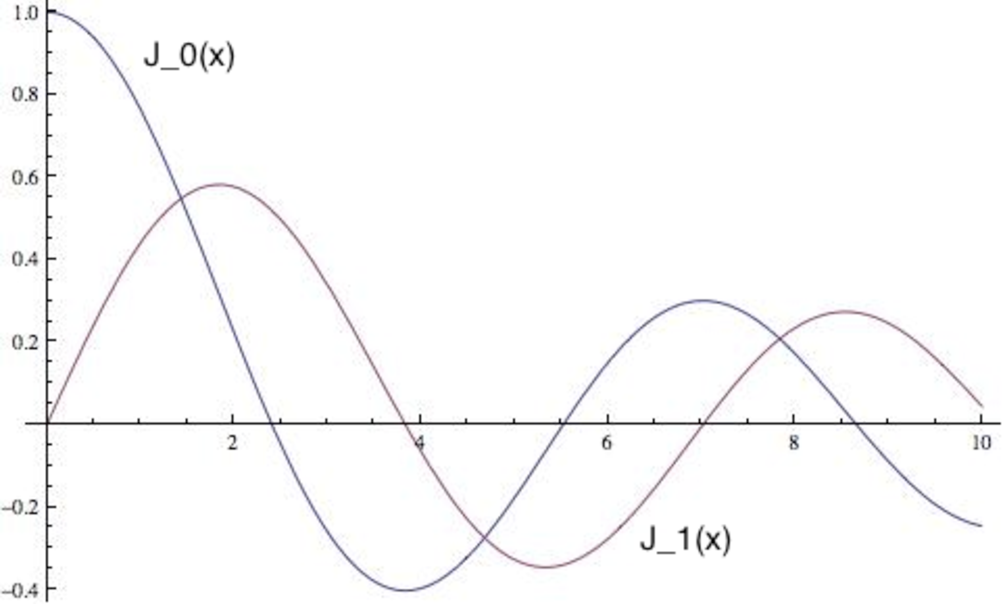
\includegraphics[width =100 mm, height = 50mm]{Bessel.pdf}
\caption{A simple plot of of J$_0$ and J$_1$ over the range that will be examined for this lab.}
\label{fig:J0J1}
\end{figure}
To generate the data for interpolations, a table of well established values will be used in increments of 1 or 0.5, depending on the technique being used.  In addition to the interesting periodic behavior of the Bessel functions, the derivatives all have a unique and valuable property.
\begin{equation}
\label{J0'}
J_0'(x) = J_1'(x)
\end{equation}
\begin{equation}
\label{Ji'}
J_i'(x) = \frac{J_{i-1}(x)-J_{i+1}(x)}{2}
\end{equation}
These facts will prove invaluable during the applications of Hermite interpolation, which requires a list of derivatives at each point in addition to the value of the function.
The physical application of this lab arises in the study of the Airy pattern.  When light passes through a circular aperture, it undergoes diffraction as a result of constructive and destructive interference.  The properties of this specific case of diffraction have been thoroughly studied and the pattern that is generated is very well understood.  The magnitude of intensity of diffracted light as a function of distance from the center of the aperture is a modified Bessel function, shown in \eqref{Airy}.
\begin{equation}
\label{Airy}
I = I_0 [\frac{2 J_1(\rho)}{\rho}]^2
\end{equation}
Using this equation and some knowledge of diffraction, one will realize that the Rayleigh criterion, which is often taught as a simple memorization of 1.22, is actually the first root of J$_1$ divided by $\pi$.  Using the root finding techniques discussed in the previous lab, the value was determined to actually be 1.219669891.
\subsection{Lagrange Interpolation}
Now that the data to be interpolated has been established, the methods to perform the interpolation itself must be examined.  Lagrange interpolation requires that only the function value at any number of points be known in order to establish an interpolating polynomial.  To derive the form of the interpolating polynomial used in the Lagrange method, one begins with a  Taylor series approximation for each of the known data points.  For purposes of interpolation, only a few terms of the series are needed, however in order to solve the system that will be generated later, the function must be replaced with an approximation $p(x)$.
\begin{equation}
\label{TaylorLagrange}
f(x_i) = p(x) + (x_i-x)p'(x) + ...
\end{equation}
Begin by considering the case of only two data points.  This provides two equations and two unknown, $p(x)$ and $p'(x)$.  If these equations are solved for $p(x)$, one finds the following:
\begin{equation}
\label{P2term}
p(x) = \frac{x-x_2}{x_1-x_2}f(x_1) + \frac{x-x_1}{x_2-x_1}f(x_2)
\end{equation}
Although this provides some valuable information for more advanced cases, the two point case is not particularly interesting.  Fortunately, it is quite easy to generalize the two point case into the case of N points.  For every additional data point, an extra term in the Taylor approximation must be used.  Repeating the above calculations, one derives the following form for N points.
\begin{equation}
\label{PNterm}
p(x) = \sum_{j=1}^N l_{j,N}(x)f(x_J)
\end{equation}
\begin{equation}
\label{LJ}
l_{j,N}(x) = \frac{(x-x_1)(x-x_2)...(x-x_{j-1})(x-x_{j+1})...(x-x_N)}{(x_j-x_1)(x_j-x_2)...(x_j-x_{j-1})(x_j-x_{j+1})...(x_j-x_N)}
\end{equation}
These two equations allow for incredibly simple computer code to interpolate very complex functions in seconds.  

Before attempting any serious applications of this method, one should note the drawbacks.  The first and most obvious drawback to this technique is that for any area outside your interpolation range, the interpolated polynomial has no correlation to the actual data.  This means that using the Lagrange polynomial to extrapolate will provide complete nonsense.   Additionally, while it would seem that increasing the number of data points would increase the accuracy of the interpolation, often times the opposite is true.  This results from the fact that these new points are farther away from the region that is important.  They, therefore, do very little to improve the accuracy in the desired region all while drastically increasing the computational time necessary to complete the interpolation.  Finally, for some well defined, evenly spaced functions, Lagrange interpolation can result in a very poor fit.  This inadequacy is best described as generating a function with many wiggles, but it is best explained visually.  A very obvious example of this error will be shown with the results.
\subsection{Hermite Interpolation}
It is clear that having additional information about data at a large distance from the region of interest is not especially helpful, but if there were a way to obtain more information within that region, it would follow that the accuracy would be increased.  For Hermite interpolation, this additional information takes the form of the derivative of the data points in the region of interest.  Consider the following third order polynomial with two data points.
\begin{equation}
\label{HermiteP}
p(x) =ax^3+bx^2+cx+d
\end{equation}
Using the same technique used in for deriving the Lagrange formulae, the following form can be obtained for our test polynomial.
\begin{eqnarray}
\label{P2term}
p(x) = \frac{[1-2\frac{x-x_1}{x_1-x_2}](x-x_2)^2}{(x_1-x_2)^2}f(x_1) + \frac{[1-2\frac{x-x_2}{x_2-x_1}](x-x_1)^2}{(x_1-x_2)^2}f(x_2) + \nonumber \\
\frac{(x-x_1)(x-x_2)^2}{(x_1-x_2)^2}f'(x_1)+\frac{(x-x_2)(x-x_1)^2}{(x_1-x_2)^2}f'(x_2)
\end{eqnarray}
Generalizing this to N points is quite a bit more complicated than the case in Lagrange interpolation but completely possible.
\begin{equation}
\label{PNtermHerm}
p(x) = \sum_{j=1}^N h_{j,N}(x)f(x_J)+\sum_{j=1}^N \bar{h}_{j,N}(x)f'(x_J)
\end{equation}
\begin{equation}
\label{HJN}
h_{j,N} = [1-2(x-x_j)l'_{j,N}(x_j)]l^2_{j,N}(x)\\
\end{equation}
\begin{equation}
\label{H_JN}
\bar{h}_{j,N} = (x-x_j)l^2_{j,N}(x)
\end{equation}
Where $l_{j,N}$ was defined in when deriving the Lagrange interpolation form.  Since Hermite interpolation also uses polynomials to fit the data, it suffers from all the same drawbacks that the Lagrange method does.
\subsection{Cubic Spline}
It is clear that, when derivatives are available, Hermite interpolation is a fast, highly accurate method.  Unfortunately, derivatives are often not available with data.  Although Lagrange interpolation is powerful, there is one significant drawback.  If one attempts to interpolate a large number of data points, the common method involves selecting a small number of points, three to four, and combining several different polynomials together piecewise.  This creates a continuous function that eliminates the drawbacks of using too many points but introduces a new issue:  the derivative of the interpolating function is no longer continuous.  
The cubic spline technique seeks to avoid this while also avoiding the other drawbacks of high order polynomial fits.  For any region $x_j \leq x \leq x_{j+1}$, the following polynomial can be defined.
\begin{equation}
\label{Pspline}
p(x) = a_j(x-x_j)^3+b_j(x-x_j)^2+c_j(x-x_j)+d_j
\end{equation}
Using the boundary conditions which require the function and its first derivative to be continuous, the coefficients can be solved for.
\begin{eqnarray}
\label{SplineCoeff}
d_j &=& f(x_j) \nonumber \\
c_j &=& \frac{p_{j+1}-p)j}{h_j} - \frac{h_j p''_{j+1} + 2h_j p''_j}{6} \nonumber \\
b_j &=& \frac{p''_j}{2} \nonumber \\
a_j &=& \frac{p''_{j+1}-p''_j}{6 h_J}
\end{eqnarray}
These coefficients indicate that the polynomial can be entirely described with only $f(x_j)$ and $p''(x_j)$.  Since the former is already known, only the second derivative is needed to complete this interpolation.  This can be solved for by considering the previous internal $x_{j-1}$.  Making use of this knowledge, a tridagonal system of equations can be found.
\[
\begin{bmatrix}
2h_1 & h_1 & & & & \\
h_1 & 2(h_1+h_2) & h_2 & & & \\
 & h+2 & 2(h_2+h_3) & h_3 & & \\
 & & & \ddots & & \\
 & & & h_{N-2} & 2(h_{N-2} + h_{N-1})& h_{N-1} \\
 & & & & h_{N-1} & 2h_{N-1} \\  
\end{bmatrix}
\begin{bmatrix}
p''_1\\
p''_2\\
p''_3\\
\vdots \\
p''_{N-1} \\
p''_N \\ 
\end{bmatrix} \]
\[ =
\begin{bmatrix}
0 \\
6\frac{p_3-p_2}{h_2} - 6\frac{p_2-p_1}{h_1}\\
6\frac{p_4-p_3}{h_3} - 6\frac{p_3-p_2}{h_2}\\
\vdots \\
6\frac{p_N-p_{N-1}}{h_{N-1}} - 6\frac{p_{N-1}-p_{N-2}}{h_{N-1}}\\
0 \\
\end{bmatrix} \]
At this point, it would be very helpful to develop a fast method for solving tridiagonal systems.  To demonstrate this method, first a general system must be developed.
\[
\begin{bmatrix}
b_1 & c_1 & & & & \\
a_2 & b_2 & c_2 & & & \\
 & a_3 & b_3 & c_3 & & \\
 & & & \ddots & & \\
 & & & a_{N-1} & b_{N-1}& c_{N-1} \\
 & & & & a_N & b_N \\  
\end{bmatrix}
\begin{bmatrix}
x_1\\
x_2\\
x_3\\
\vdots \\
x_{N-1} \\
x_N \\ 
\end{bmatrix}
=
\begin{bmatrix}
r_1\\
r_2\\
r_3\\
\vdots \\
r_{N-1} \\
r_N \\ 
\end{bmatrix}
 \]
With a bit of clever manipulation, one can determine the following for an incremental equation for the solutions to the above matrix.
\begin{equation}
\label{Tridiag}
x_{N-j} = \frac{\rho_{N-j}-c_{N-j}x_{N-j+1}}{\beta_{N-j}} \text{     } j=1,...,N-1
\end{equation}
\begin{equation}
\label{TridiagCoeff}
\beta_j = b_j - \frac{a_j}{\beta_{j-1}}c_{j-1}  \text{ and } \rho_j = r_j-\frac{a_j}{\beta_{j-1}}\rho_{j-1} \text{    }j=1,...,N-1
\end{equation}
\begin{equation}
\label{TridiagInitCoeff}
\beta_1 = b_1 \text{ and } \rho_1 = r_1
\end{equation}
Now that an effective algorithm for solving tridiagonal systems has been derived, the cubic spline fitting is a simple application of this to the system that was derived earlier.
\subsection{Derivative Approximations}
It is clear from the complexity of the spline fits that it is preferable to use Hermite interpolation whenever possible.  Numerical approximations to a function's derivative allow for this quite well.  Beginning with the definition of a derivative, the following approximations can be made, which is known as the forward difference approximation.
\begin{equation}
\label{ForDiff}
f'_h(x)=\frac{f(x+h)-f(x)}{h}
\end{equation}
This approximation can be confirmed by performing a Taylor expations of $f(x+h)$ about $f(x)$ and solving for $f'(x)$.  From this expansion, it is found that the error is of order $h$.   Additionally, the backwards difference approximation can be obtained with the same method and same error to be
 \begin{equation}
\label{BackDiff}
f'_h(x)=\frac{f(x)-f(x-h)}{h}
\end{equation}
In the forward difference approximation, the first error term is negative while in the backwards it is positive.  This implies that if one were to combine the two, the first order error terms would cancel, leaving an error of order $h^2$.  This is called the central difference approximation and takes the following form
\begin{equation}
\label{CentDiff}
f'_h(x)=\frac{f(x+h)-f(x-h)}{2h}
\end{equation}
Sometimes one needs to find second derivatives as well.  The same methods can be applied multiple times to evaluate higher order derivatives.  Applying the central difference method twice, one obtains \eqref{CentDiff2} which also has error on the order of $h^2$.
\begin{equation}
\label{CentDiff2}
f''_h(x)=\frac{f(x+h)-2f(x)+f(x-h}{h^2}
\end{equation}
A similar application of the forward difference method yields \eqref{ForDiff2}, with an error of order $h$.
\begin{equation}
\label{ForDiff2}
f''_h(x)=\frac{f(x)-2f(x+h)+f(x+2h)}{h^2}
\end{equation}
The final and most complicated method for finding a derivative approximation is called Richardson extrapolation.  Above it was shown that combining two different expressions can eliminate error terms.  Richardson extrapolation seeks to do this with only one term.  This goal is achieved by applying the central difference method twice, using two different step sizes.
\begin{equation}
\label{CentDiffRich1}
f'_h(x)=\frac{f(x+h)-f(x-h)}{2h}-\frac{h^2}{6}f'''(x)+...
\end{equation}
Now the process is repeated with a step of $h^* = 2h$
\begin{equation}
\label{CentDiffRich2}
f'_h(x)=\frac{f(x+2h)-f(x-2h)}{4h}-\frac{4h^2}{6}f'''(x)+...
\end{equation}
If one divides \eqref{CentDiffRich2} by 4 and subtracts it from \eqref{CentDiffRich1}, the following is obtained
\begin{equation}
\label{CentDiffRich}
f'_h(x)=\frac{f(x-2h)-8f(x-h)_8f(x+h)-f(x+2h)}{12h} + O(h^4)
\end{equation}
This form of Richardson extrapolation allows one to calculate "new" values, but it can also be used recursively to obtain an incredibly accurate value for a single expression.  Instead of performing the extrapolation numerically, consider the effect of a symbolic approach.  Begin with $D_1(h)$ and $D_1(2h)$, the numerical approximations to the derivative using step size $h$ and $2h$, respectively.  The error for this method is dependent on the square of the step size, meaning that $D_1(2h)$ has four times the error of $D_1(h)$.  Now define a new approximation, $D_2(h)$, which is the difference of the first two approximations.  
\begin{equation}
\label{CentDiffRich}
D_2(h)=D_1(h)-[\frac{D_1(2h)-D_1(h)}{2^2-1}] = \frac{4D_1(h)-D_1(2h)}{3}
\end{equation}
This term has an error on the order of $h^4$, since the second order error was eliminated via subtraction.  This process can be repeated until the desired accuracy level is reach with this recursive relationship.
\begin{equation}
\label{CentDiffRich}
D_{i+1}(h)=\frac{2^{2i}D_i(h)-D_i(2h)}{2^{2i}-1}
\end{equation}
\subsection{Linear Least Squares}
Now that interpolation has been thoroughly explored, it would be wise to consider the alternative.  Data fitting provides a way to calculate values between data points when the data has variance, such as real experimental data.  To begin, a simple linear fit will be explored using a guess function.
\begin{equation}
\label{Line}
g(x)=a+bx
\end{equation}
An expression for the error from the measured data, $y_i$, must be established.
\begin{equation}
\label{LineError}
S=\sum_{i=1}^N (g(x_i)-y_i)^2
\end{equation}
To find the best fit, this error must be minimized.  This occurs when the first derivative is zero and the second derivative is positive.  Applying these conditions, one discovers the following.
\begin{eqnarray}
\label{LineSolution}
aN+b\sum_{i=1}^N x_i &=& \sum_{i=1}^N y_i \\
a\sum_{i=1}^N x_i + b\sum_{i=1}^N x^2_i &=& \sum_{i=1}^N x_i y_i
\end{eqnarray}
As was the case with previous test cases, this linear approximation can easily be generalized to higher order fits.  For an $m$ order polynomial, one can derive the system below.
\[
\begin{bmatrix}
N & \sum x_i &\sum x^2_i &... &\sum x^m_i \\
\sum x_i &\sum x^2_i & \sum x^3_i &...& \sum x^{m+1}_i \\
 \vdots& \vdots & \vdots & &\vdots \\
\sum x^m_i &\sum x^{m+1}_i &\sum x^{m+2}_i & ... & \sum x^{m+m}_i \\
\end{bmatrix}
\begin{bmatrix}
c_0\\
c_1\\
\vdots\\
c_m \\ 
\end{bmatrix}
=
\begin{bmatrix}
\sum y_i\\
\sum y_ix_i\\
\vdots \\
\sum y_ix^m_i \\
\end{bmatrix}
 \]
To solve this, another matrix solving technique must be used, since this matrix is not tridiagonal.  The method that will be used for this purpose is call LU decomposition.  The basis of this method is the conversion of a general matrix into a product of an upper and lower triangular matrices.  Beginning with the original matrix equation
\begin{equation}
\label{Axb}
\text{Ax}=\text{b}
\end{equation}
A can be replaced with LU, the product of two triangular matrices, and then Ux with z, leaving
\begin{equation}
\label{Lzb}
\text{Lz}=\text{b}
\end{equation}
At this point, some simple matrix manipulations will allow one to solve for z.
\begin{equation}
\label{z}
z_i=\frac{b_i-\sum_{k=1}^{i-1} l_{ik}z_k}{l_{ii}} \text{,          }i=2,...,N
\end{equation}
Now that z is know, a few more simple matrix operations will provide x. 
\begin{equation}
\label{x}
x_{N-i}=z_{N-i} - \sum_{k=N-i+1}^N u_{N-i,k} x_k \text{,    }i=1,...,N-1
\end{equation}
Now, all the tools necessary to perform a general linear least squares fit are available.  Applying LU decomposition to the sums of the data points as described in the matrix derived with the method is a trivial task.
\subsection{Non-Linear Least Squares}
The final method to be explored in this lab is the applications of least squares fitting to non-linear systems.  To begin this method of fitting, a function is developed that depends on a series of unknown parameters.  The least squares error is given as
\begin{equation}
\label{nonlinerror}
S(a_1,a_2,...,a_m)=\sum_{k=1}^N (y_k- Y(x_k;a_1,a_2,...,a_m))^2
\end{equation}
The goal is to minimize S and in practice that is done by varying the parameters $a_i$ in a systematic way until the minimum is found.  One must begin with an initial guess of each parameter which implies that the error, $S$, will be quadratic.  By evaluating $S$ at the initial guess $a_i^0$ and a small step $h_1$ above and below that value, one finds that the improved value for the parameter is
\begin{equation}
\label{parameter}
a_i^1=a_i^0 - \frac{h_1}{2} \frac{S(a_i^0+h_1,...)-S(a_i^0-h_1,...)}{S(S(a_i^0+h_1,...)-2S(a_i^0,...)+S(a_i^0-h_1,...)}
\end{equation}
This formula can be applied to each parameter to generate very good guesses for each parameter.
\section{Applications}
\subsection{Exercise 3.2}
The first exercise in this lab is the analysis of some of the drawbacks of Lagrange interpolation.  The goal of this exercise is to fit \eqref{tanh} to illustrate the 'wiggles' that can occur when using high order polynomials
\begin{equation}
\label{tanh}
f(x) = \frac{1+\text{tanh}(2\alpha x)}{2}
\end{equation}
\begin{figure}[!h]
\centering
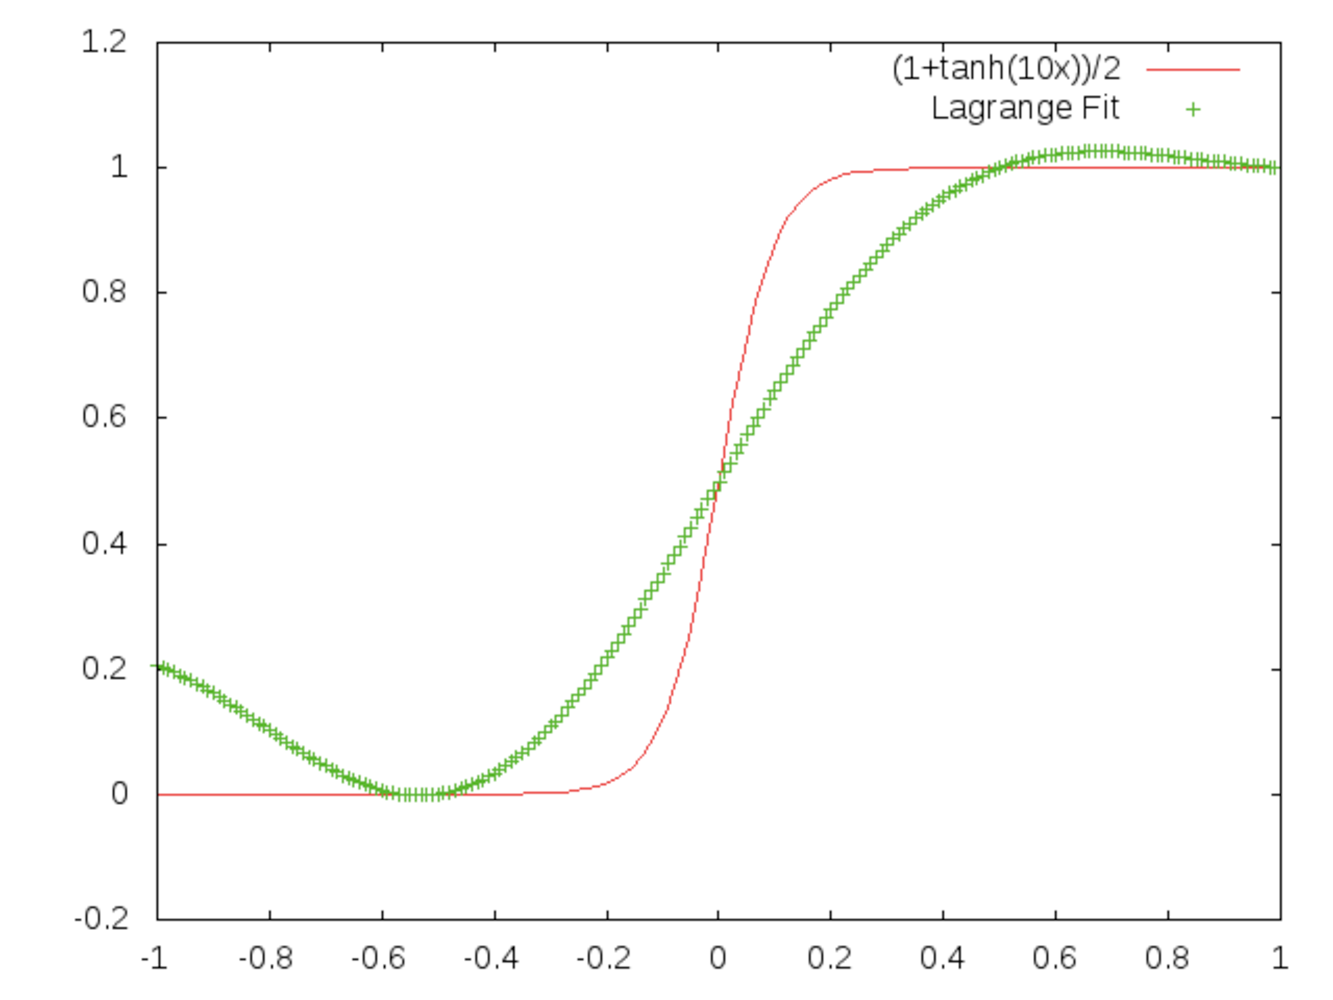
\includegraphics[width =120 mm, height = 90mm]{Ex_3_2.pdf}
\caption{An example of the a failed 21 point interpolation of \eqref{tanh}.}
\label{fig:3.2}
\end{figure}
The data points used to fit \eqref{tanh} ranged from -10 to 10, while the region of interest was only between -1 and 1.  That means that, while the interpolation passes through the known points at -0.5, 0, and 0.5, every point between them is incorrect.  The 'wiggles' are also quite apparent in Figure \ref{fig:3.2}.
\subsection{Exercise 3.3, 3.4, and Airy Patterns}
The next focus of study is the interpolation of Bessel functions to develop the Airy pattern.  Beginning with Lagrange interpolation, the first two Bessel functions, $J_0(x)$ and $J_1(x)$, were interpolated.
\begin{figure}[!h]
\centering
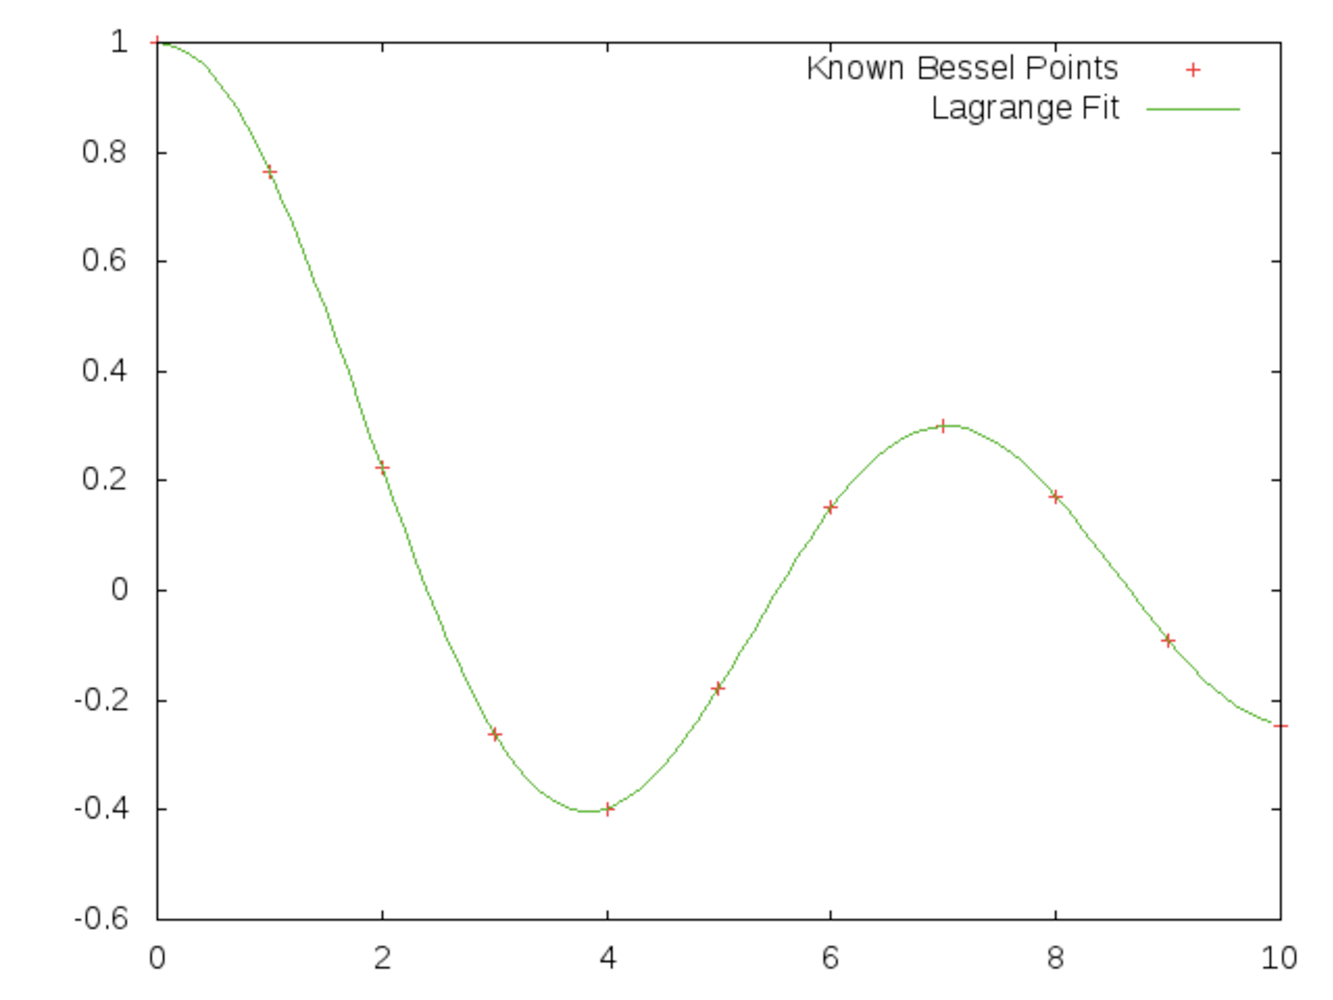
\includegraphics[width =120 mm, height = 80mm]{Ex_3_3_j0.pdf}
\caption{Lagrange interpolation of $J_0(x)$.}
\label{fig:3.3.j0}
\end{figure}
\begin{figure}[!h]
\centering
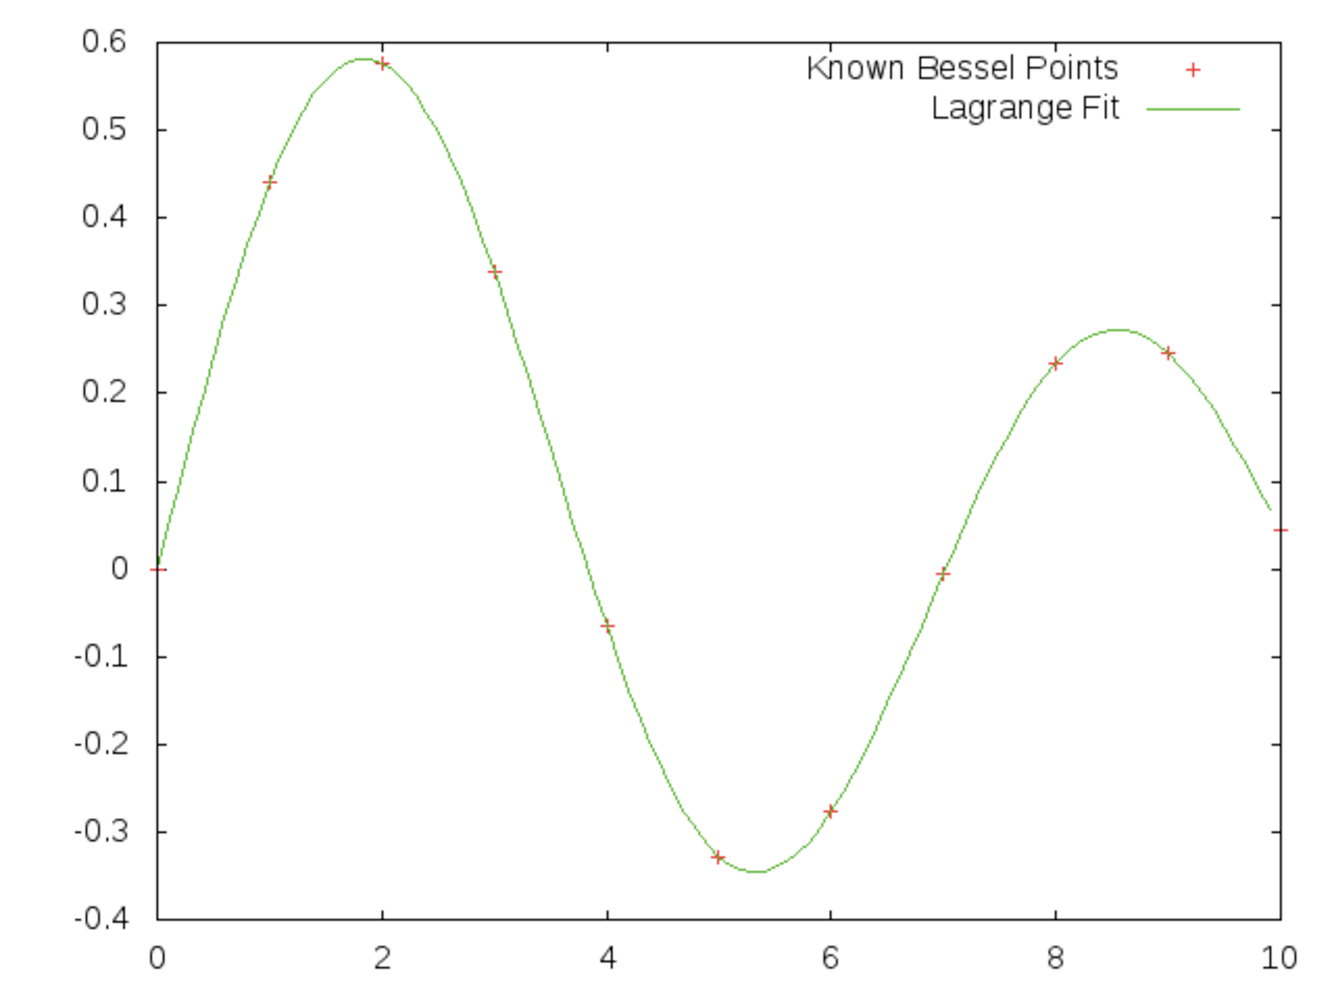
\includegraphics[width =120 mm, height = 80mm]{Ex_3_3_j1.pdf}
\caption{Lagrange interpolation of $J_1(x)$.}
\label{fig:3.3.j1}
\end{figure}
Both interpolations used all data points available so one might expect the results to have a low level of accuracy.  For comparison, another interpolation was performed on $J_0(x)$ using only three points.  To compare the accuracy of using 21 points versus 3, a table is included to show $J_0(2.3)$.
\begin{figure}[!h]
\centering
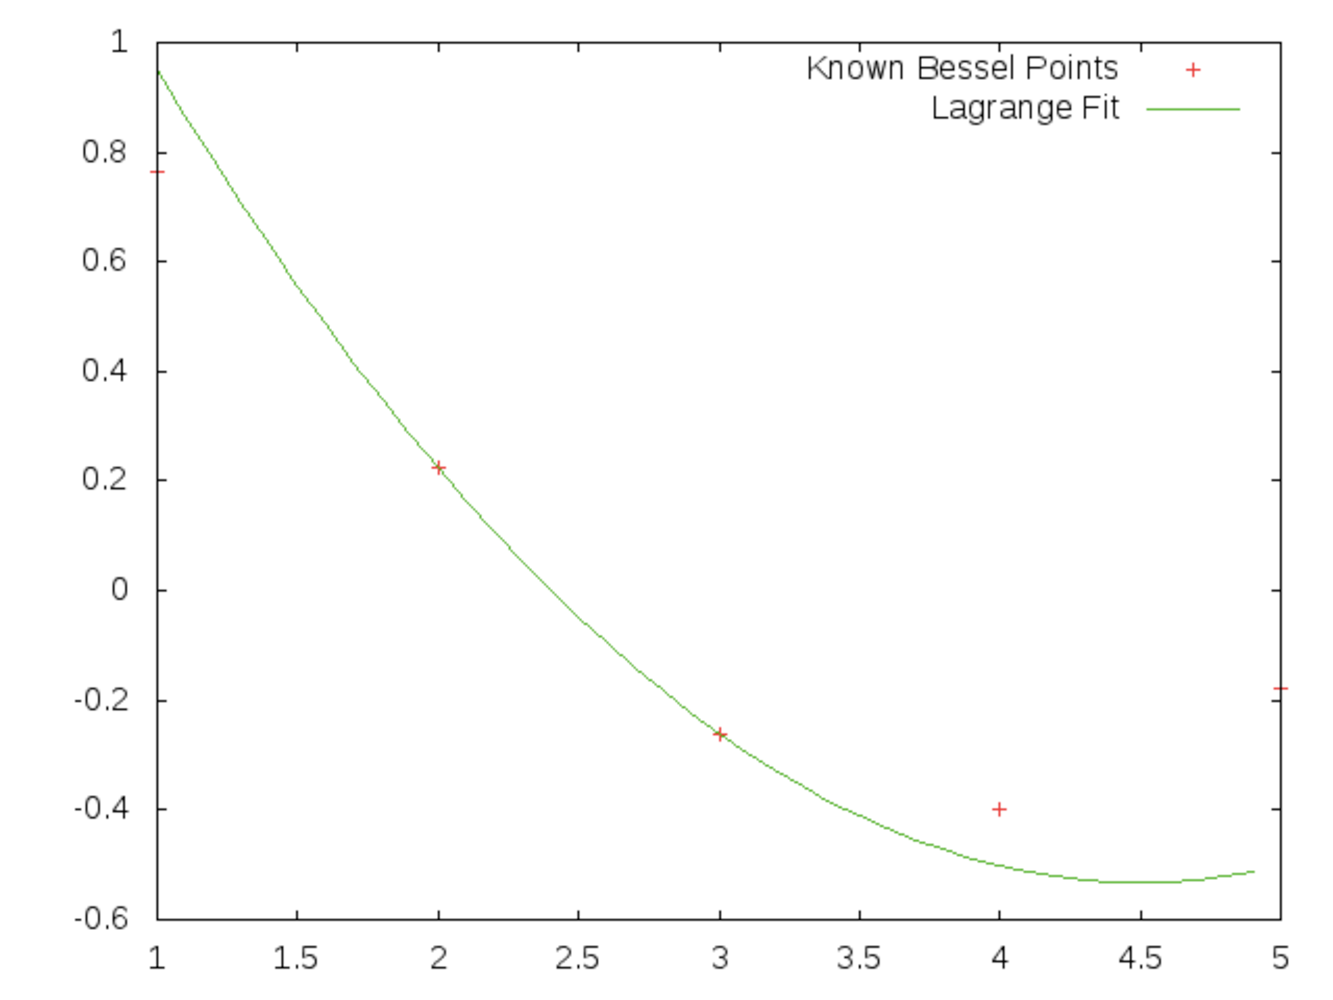
\includegraphics[width =120 mm, height = 65mm]{Ex_3_3_3point.pdf}
\caption{Lagrange interpolation of $J_0(x)$ using $x$ values of 2.0, 2.5, and 3.0.}
\label{fig:3.3.j0}
\end{figure}
\begin{center}
Table 1:  21 Point VS 3 Point Interpolation - $J_0(2.3)$ \\
\begin{tabular}{ | c | c | c |}
\hline
Table Value &  21 Point & 3 Point  \\ \hline
0.0555397844 & 0.055540 & 0.053253 \\ \hline
\end{tabular}
\end{center}
The comparison of the 21 point interpolation with the 3 point interpolation indicates that there is actually higher accuracy when using a larger number of points.  It is likely that this is the exception and not the rule, since the consequences of high order polynomials have already been proven.

The final goal using Lagrange interpolation was to generate an Airy pattern from \eqref{Airy}.
\begin{figure}[h!]
\centering
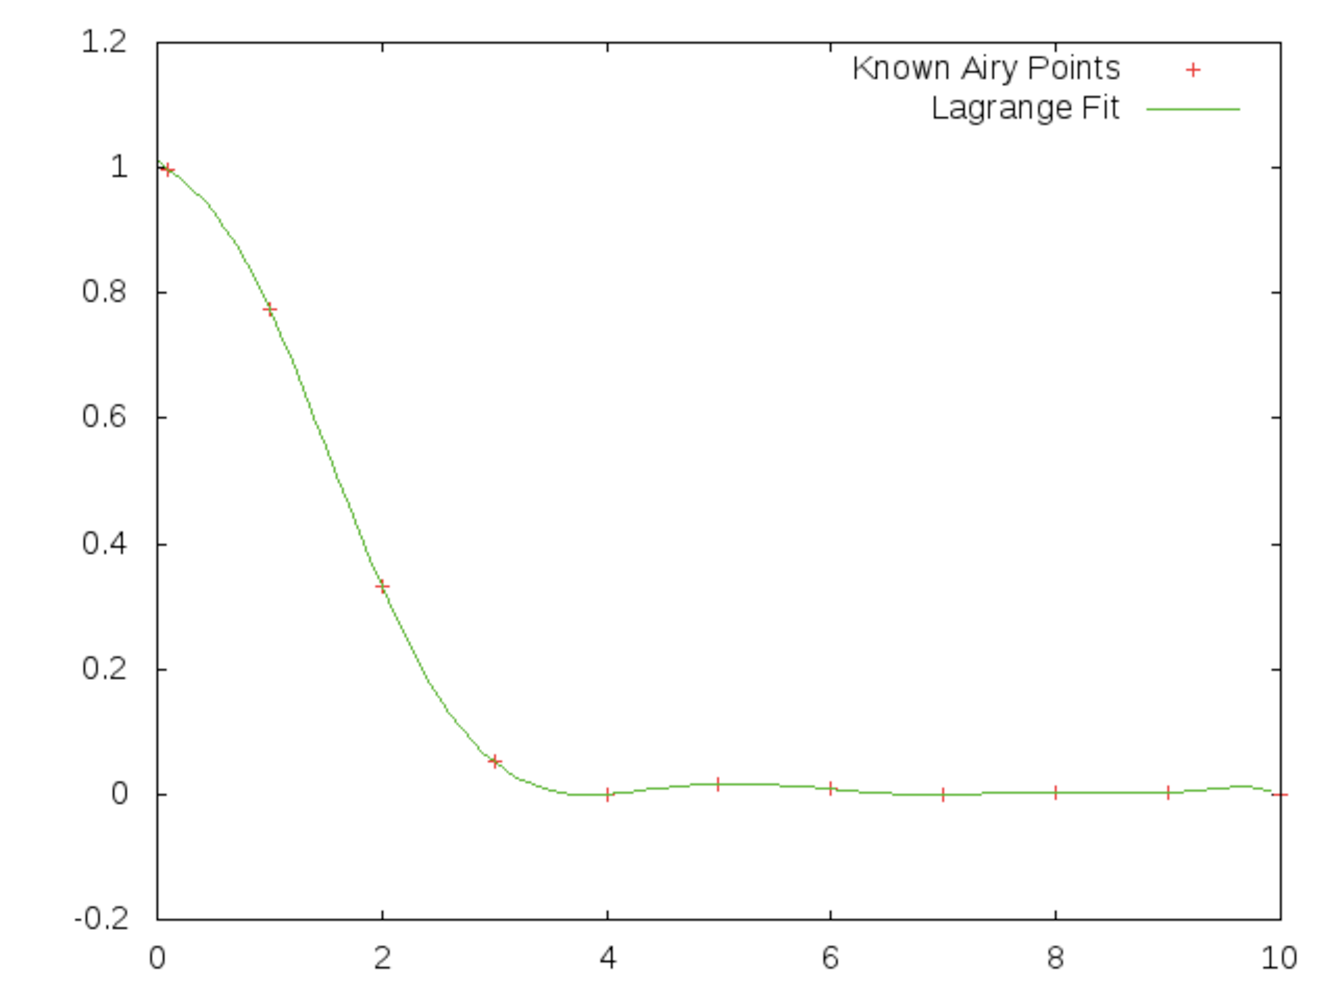
\includegraphics[width =120 mm, height = 65mm]{Ex_3_3_airy.pdf}
\caption{Lagrange interpolation of \eqref{Airy}, also known as the Airy pattern.}
\label{fig:3.3.airy}
\end{figure}
The Airy pattern represents the intensity of light after passing through a circular aperture as a function of distance from the center.  Figure \ref{fig:3.3.airy} represents this quite well, with a value of 1 (full intensity) at the origin followed by a decay to a minimum and then oscillating 'fringes' at high radii.  As mentioned in the Section 1.1, the Airy pattern is useful for performing diffraction calculations, and the Rayleigh criterion can be derived from this plot.  The first zero of the Airy pattern divided by $\pi$ is 1.219669891, which is quite close to the standard 1.22 used in most cases.  

Now, the same problems will be explored using Hermite interpolation.  From a visual inspection, the results look identical to those of the Lagrange interpolation.
\begin{figure}[!h]
\centering
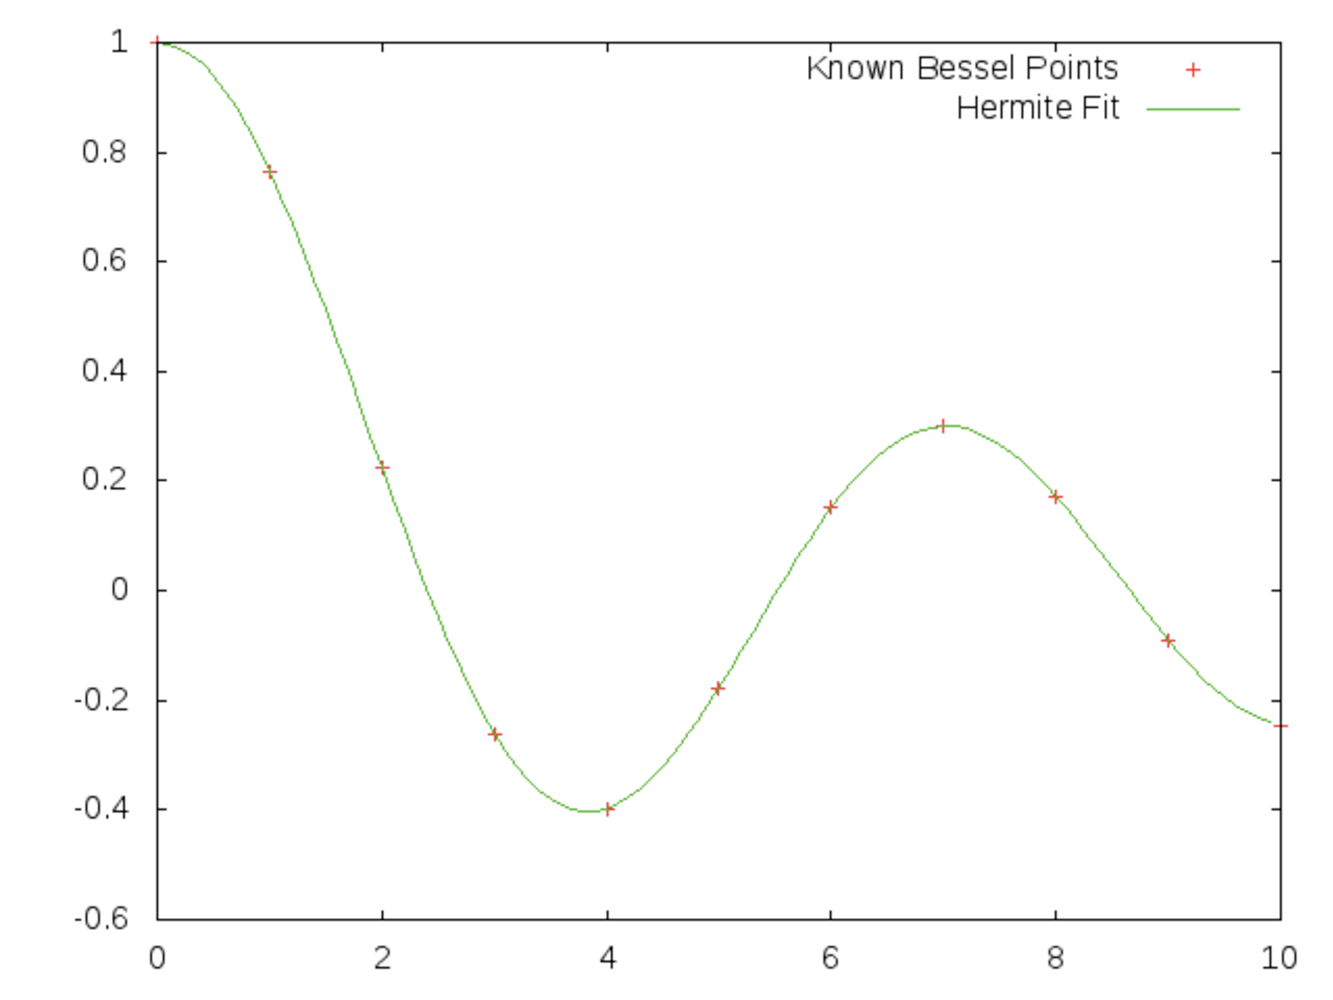
\includegraphics[width =120 mm, height = 70mm]{Ex_3_4_j0.pdf}
\caption{Hermite interpolation of $J_0(x)$.}
\label{fig:3.3.j0}
\end{figure}
\begin{figure}[!h]
\centering
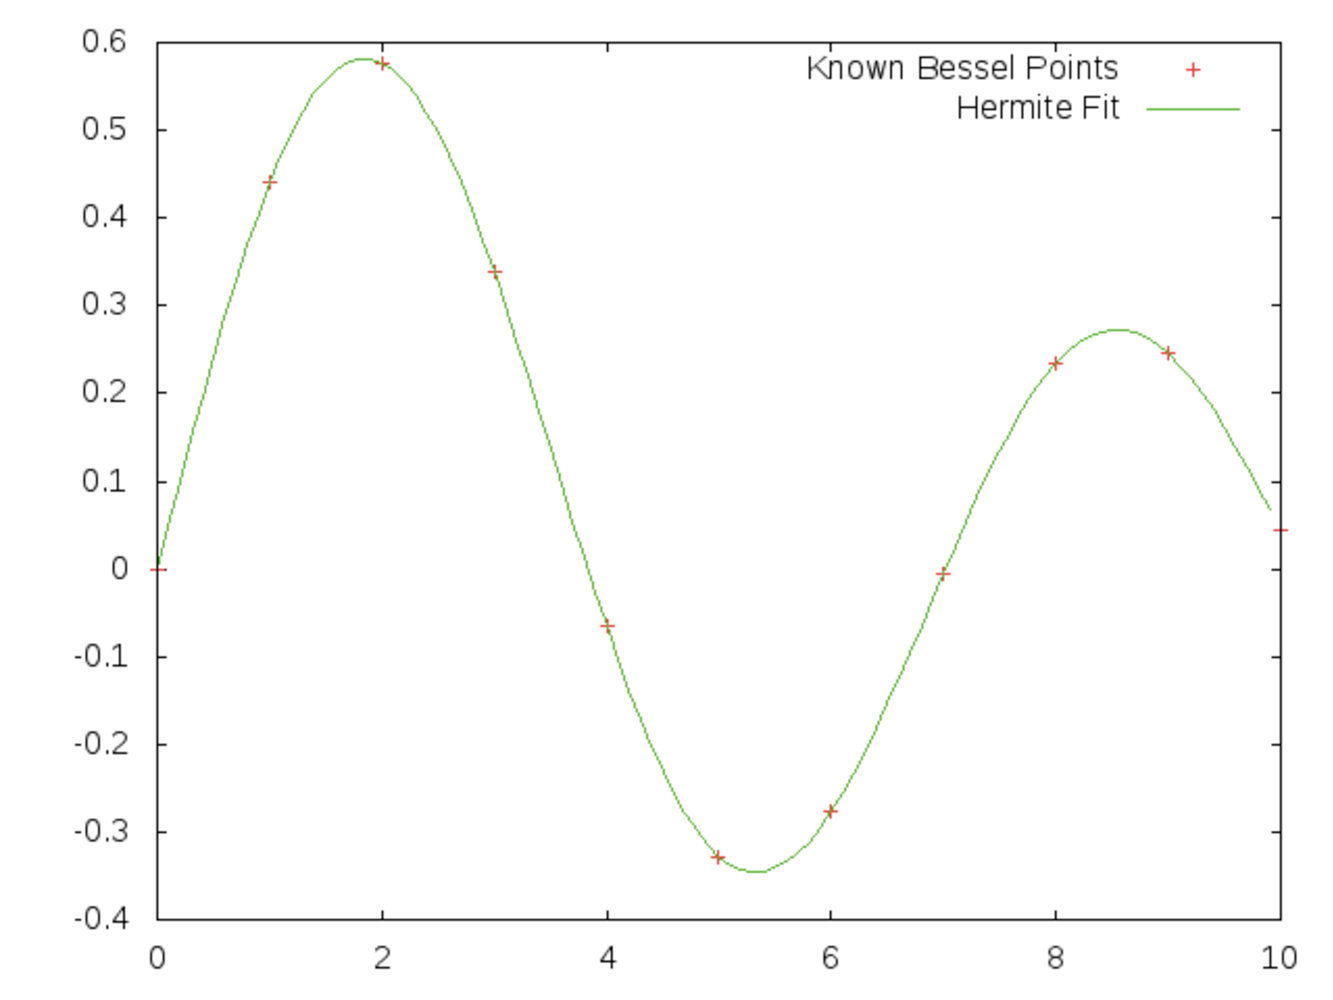
\includegraphics[width =120 mm, height = 70mm]{Ex_3_4_j1.pdf}
\caption{Hermite interpolation of $J_1(x)$.}
\label{fig:3.3.j1}
\end{figure}
To gain a more quantitative comparison, a few values of $J_0(x)$ and $J_1(x)$ calculated from both the Lagrange and Hermite method are included in Table 2.
\begin{center}
Table 2:  Hermite VS Lagrange Interpolation \\
\begin{tabular}{ | c | c | c | c |}
\hline
 & Table Value & Hermite & Lagrange  \\ \hline
$J_0(1.3)$ & 0.6200859896 & 0.620086 & 0.620086 \\ \hline
$J_1(1.3)$ & 0.5220232474 & 0.522025 & 0.522023 \\ \hline
$J_0(8.3)$ & 0.0960061009 & 0.096006 & 0.096006 \\ \hline
$J_1(8.3)$ & 0.265739302 & 0.265738 & 0.265739 \\ \hline
\end{tabular}
\end{center}
From these selected values, it appears that the Lagrange method actually offers superior accuracy over the Hermite.  

Finally, the Airy pattern was interpolated using the Hermite method.  
\begin{figure}[h!]
\centering
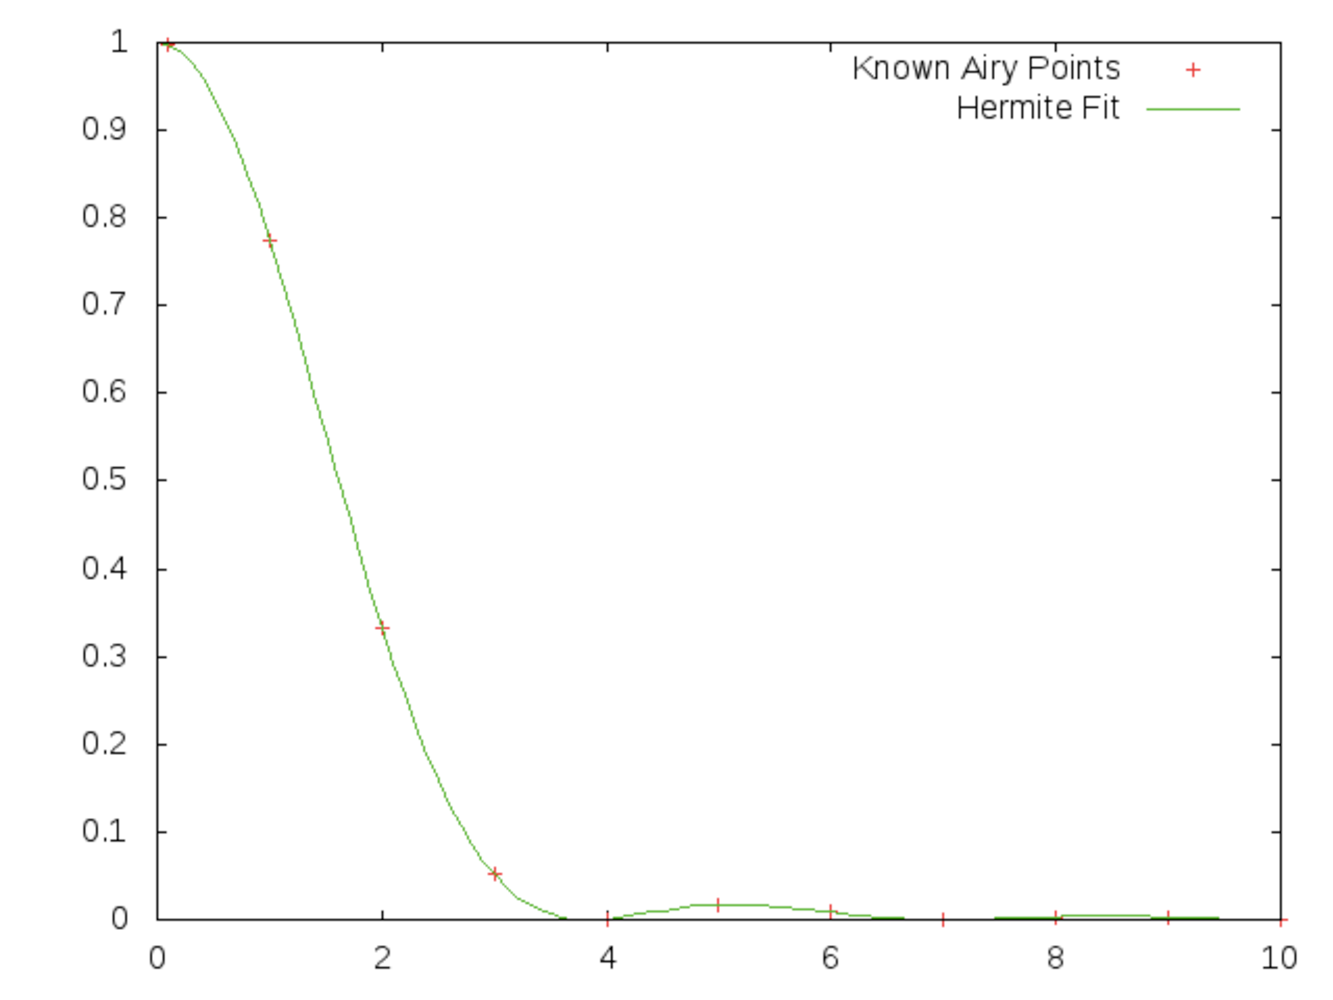
\includegraphics[width =120 mm, height = 65mm]{Ex_3_4_airy.pdf}
\caption{Hermite interpolation of \eqref{Airy}, also known as the Airy pattern.}
\label{fig:3.4.airy}
\end{figure}
This data also matches the expected values to a high level of accuracy.  
\subsection{Exercise 3.5 and 3.6 - Cubic Spline}
In preparation for Cubic Spline interpolation, the algorithm developed in Section 1.4 for solving tridiagonal systems must be tested.  The TriSolve method was tested on the following matrix.
\[
\begin{bmatrix}
2 & -1&0 &0 &0 \\
-1 &2& -1 &0& 0 \\
 0& -1& 2& -1&0 \\
0 &0 &-1 & 2 & -1 \\
0&0 &0 &-1 & 2 \\
\end{bmatrix}
\begin{bmatrix}
x_1\\
x_2\\
x_3\\
x_4 \\
x_5 \\ 
\end{bmatrix}
=
\begin{bmatrix}
0\\
1\\
2 \\
3 \\
4 \\
\end{bmatrix}
 \]
The solution to this system was found to be.
\begin{eqnarray}
\label{3.5}
x_1 &=& 3.333333 \nonumber \\
x_2 &=& 6.666667\nonumber \\
x_3 &=& 9.000000\nonumber \\
x_4 &=& 9.333333\nonumber \\
x_5 &=& 6.666667
\end{eqnarray}
These solutions match the analytic solutions perfectly.

Now, this technique can be applied to Cubic Spline fitting.  As a test, the $J_1(x)$ Bessel function was fit using the spline method.
\begin{figure}[!h]
\centering
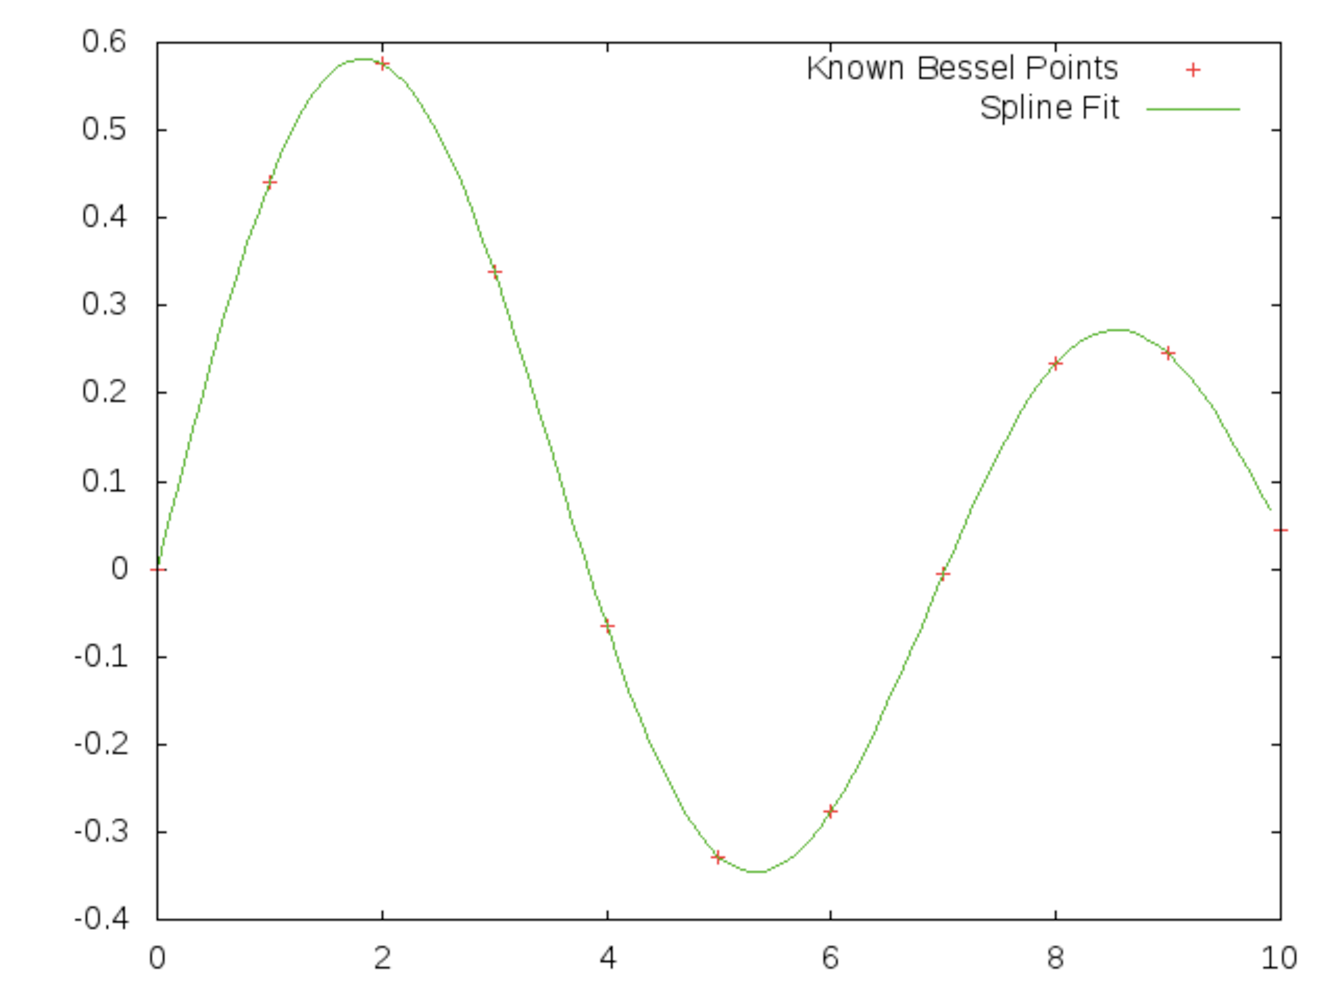
\includegraphics[width =120 mm, height = 70mm]{Ex_3_6.pdf}
\caption{Cubic Spline interpolation of $J_1(x)$.}
\label{fig:3.6}
\end{figure}
A comparison similar to that done in Table 2 indicates that this fit has an even lower accuracy than the Hermite method.  
\begin{center}
Table 3:  Cubic Spline VS Lagrange Interpolation \\
\begin{tabular}{ | c | c | c | c |}
\hline
 & Table Value & Cubic Spline & Lagrange  \\ \hline
$J_1(1.3)$ & 0.5220232474 & 0.523776 & 0.522023 \\ \hline
$J_1(8.3)$ & 0.265739302 & 0.265179 & 0.265739 \\ \hline
\end{tabular}
\end{center}
Finally, using the root finding techniques developed in the previous lab, the root of $J_1(x)$ was found to be 3.831705970.
\subsection{Exercise 3.13 and Richardson Extrapolation}
To begin the applications of numerical derivative approximations, a function must be selected.  For this lab, this function will be explored
\begin{equation}
\label{xex}
f(x)=x e^x
\end{equation}
\begin{figure}[!h]
\centering
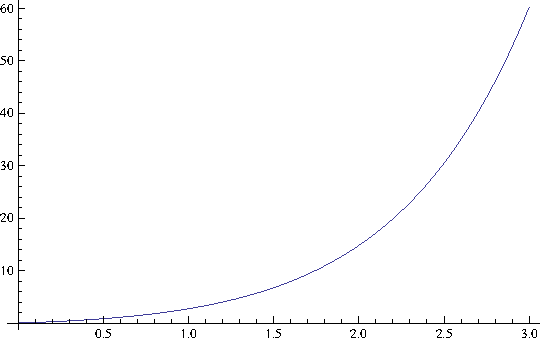
\includegraphics[width =100 mm, height = 45mm]{Ex_3_13.pdf}
\caption{A visual representation of Eq. \eqref{xex}.}
\label{fig:3.13}
\end{figure}
First, the simple forward, central, and backwards difference techniques were applied to find $f'(x)$.  The main purpose of this application was to verify the order of error in each technique.  The errors that were predicted for each technique can clearly bee seen if Figure \ref{fig:3.13.1st}.  The forwards and backwards both have a linear dependence on step size while the central is more well described as a quadratic function.
\begin{figure}[!h]
\centering
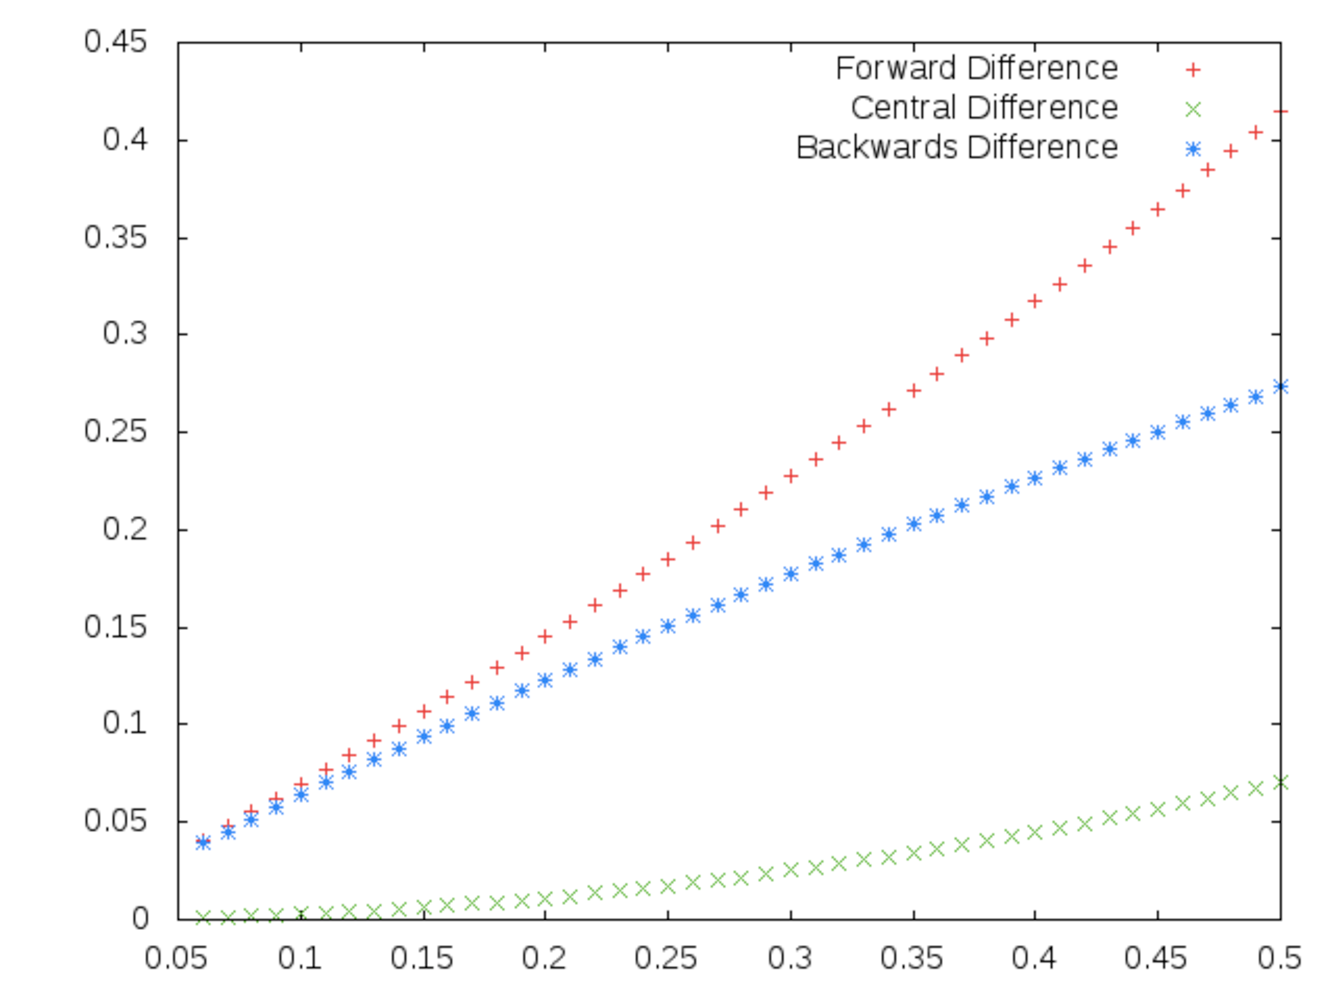
\includegraphics[width =120 mm, height = 60mm]{Ex_3_13_1st.pdf}
\caption{A plot of step size versus error of the first derivative of $f(2)$.  Note that the forward and backwards difference methods have a much greater error than the central difference method.}
\label{fig:3.13.1st}
\end{figure}
\begin{figure}[!h]
\centering
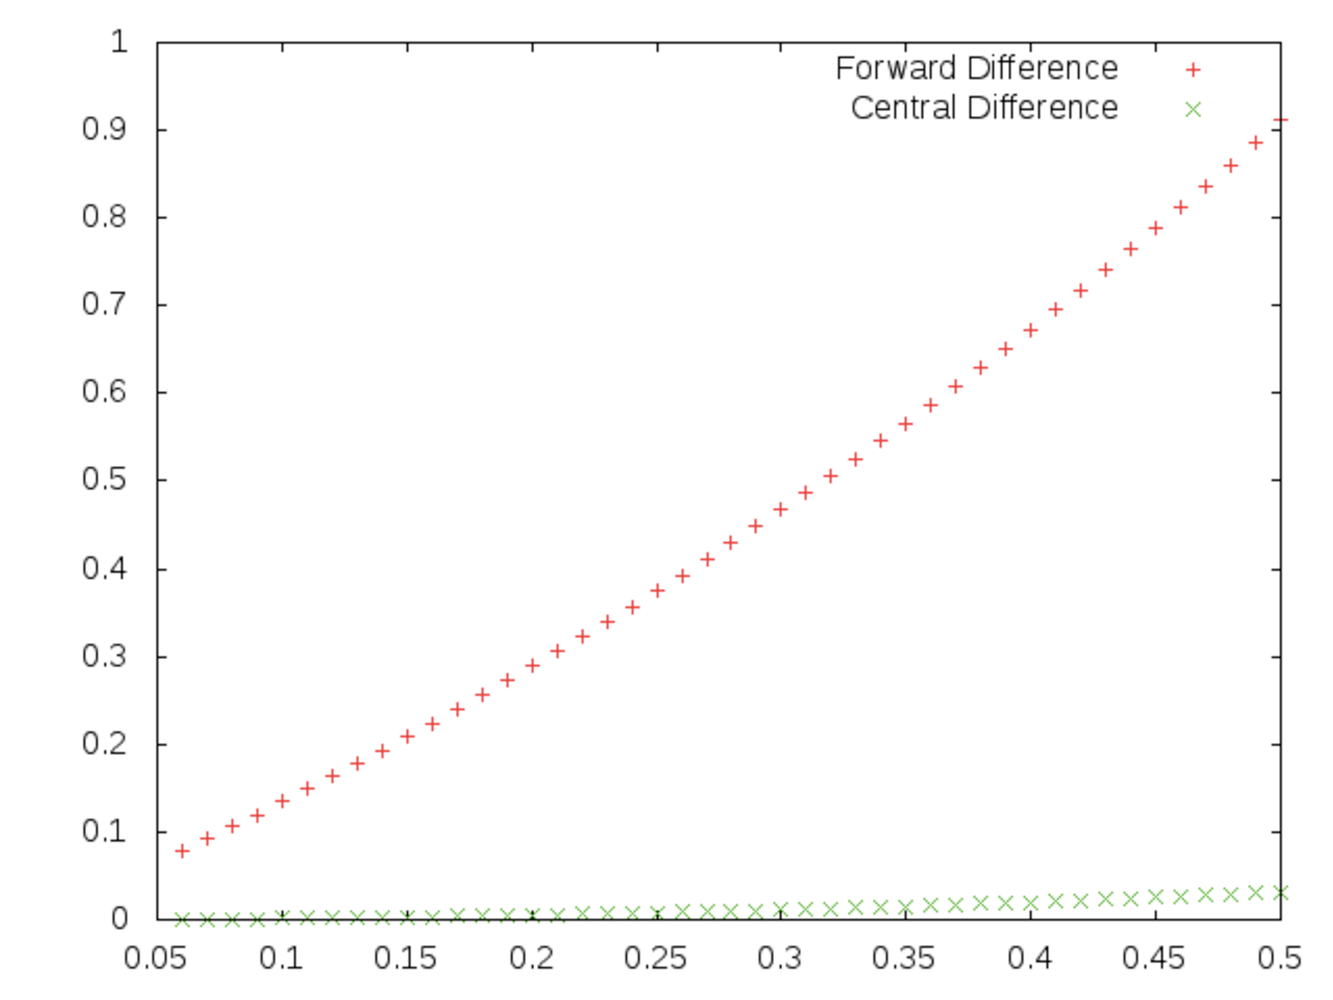
\includegraphics[width =120 mm, height = 60mm]{Ex_3_13_2nd.pdf}
\caption{A plot of step size versus error of the second derivative of $f(2)$.  Note that the forward difference methods has a much greater error than the central difference method.}
\label{fig:3.13.2nd}
\end{figure}

Next, the second derivative of \eqref{xex} was calculated using the forward and central difference methods derived for second order derivatives.  Again, the error was examined to confirm the predictions made earlier.  Figure \ref{fig:3.13.2nd} confirm that the forward difference technique has error on the order of $h$ while the central method has order of $h^2$.

Finally, Richardson extrapolation was applied to \eqref{xex}.  This application resulted in the following solution.
\begin{center}
Table 4:  Richardson Extrapolation of $f'(2)$ \\
\begin{tabular}{ | c | c | c | c | c |}
\hline
h & $D_1$ & $D_2$ & $D_3$ & $D_4$ \\ \hline
0.400 & 23.163464 &  &  &  \\ \hline
0.200 & 22.414161 & 22.164393 &  &  \\ \hline
0.100 & 22.228787 & 22.166996 & 22.167169 & \\ \hline
0.050 & 22.182565 & 22.167158 & 22.167168 & 22.167168 \\ \hline
\end{tabular}
\end{center}
Additionally, Richardson extrapolation was used to solve for $f''(2)$, which was found to be 29.55622440.
\subsection{Exercise 3.17 and 3.20 - Linear Least Squares}
Before any proper data fitting can occur with the least squares method, it must be proven that the LU decomposition algorithm derived earlier works.  To test this technique, the tridiagonal matrix that was solved above was used.  Since the answers have already been determined, this makes an excellent test case.  Fortunately, the solution for this system obtain with LU decomposition match the analytic and TriSolve solutions perfectly.

To properly test the least squares method that was developed, a set of fictional data of a particle moving under the influence of gravity was prepared.  Using least squares fitting, a second order polynomial was developed to represent this data.
\begin{equation}
\label{gravityFit}
p(x) = 1.654167 + 3.902567 x -5.202040x^2
\end{equation}
Applying some background knowledge of the equations of motion, an approximation for $g$ can be found by doubling the coefficient on the squared term.  This approximation is $10.4041 \frac{\text{m}}{\text{s}^2}$.
\begin{figure}[!h]
\centering
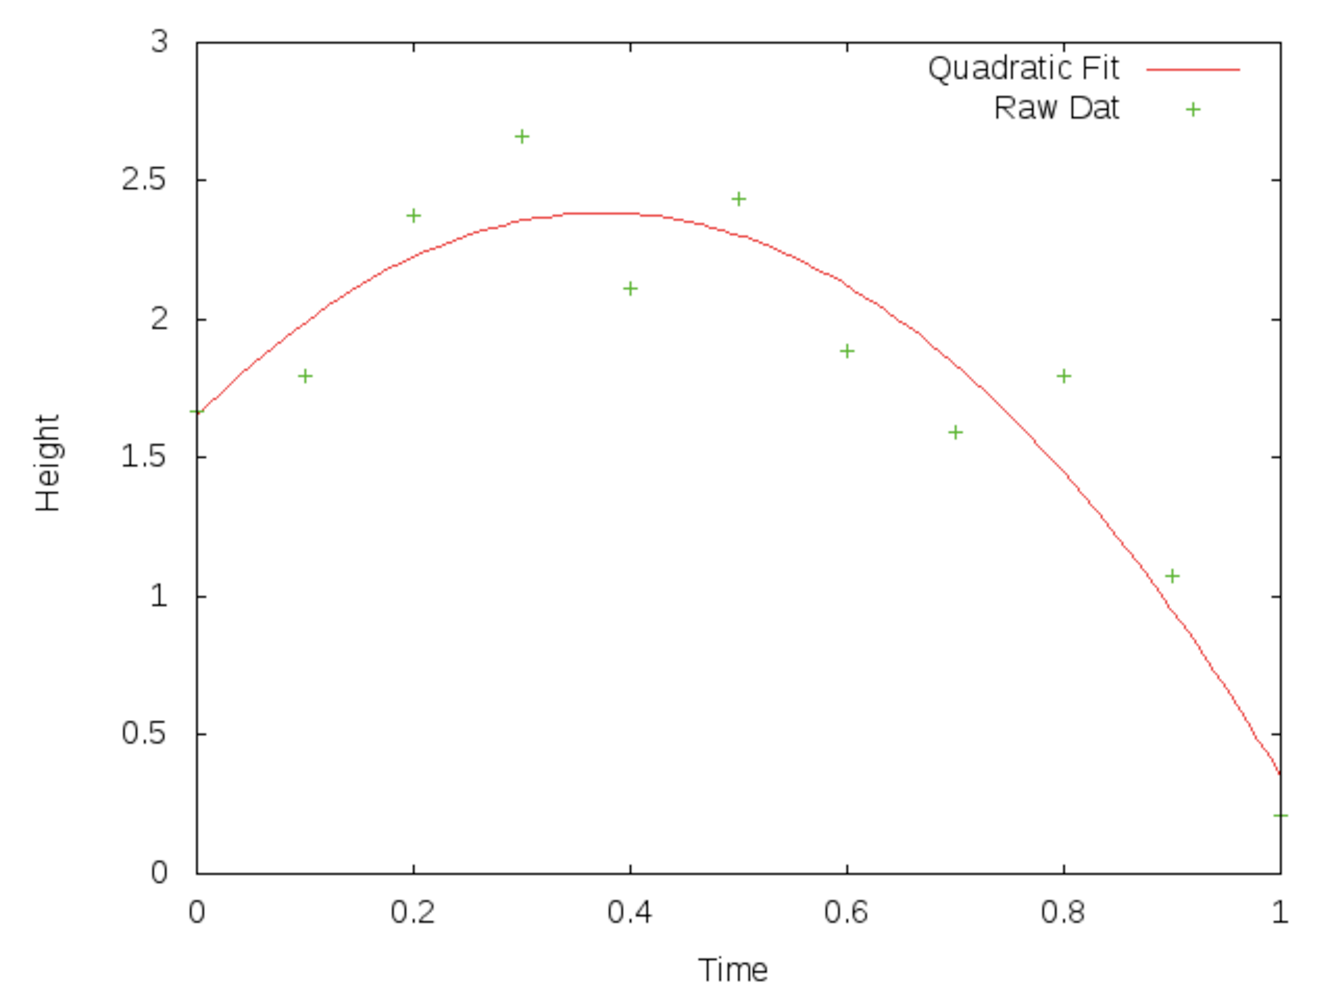
\includegraphics[width =120 mm, height = 70mm]{Ex_3_20.pdf}
\caption{A fit of fictional position vs time data using linear least squares.}
\label{fig:3.20}
\end{figure}
\subsection{Exercise 3.21}
The final application of this lab's techniques is the fitting of a non-linear data set based upon the light emitted by an excited atom.  This data can be described by a Lorentzian linshape of the following form
\begin{equation}
\label{lorentz}
I(\lambda) = I_0 \frac{1}{1+4(\lambda-\lambda_0)^2 /  \Gamma^2}
\end{equation}
Equations \eqref{lorentz} provides an excellent starting point for the fit, and has four obvious parameters: $I_0$, $\lambda_0$, $\Gamma$, and a baseline shift we will define as $B$.
\begin{figure}[!h]
\centering
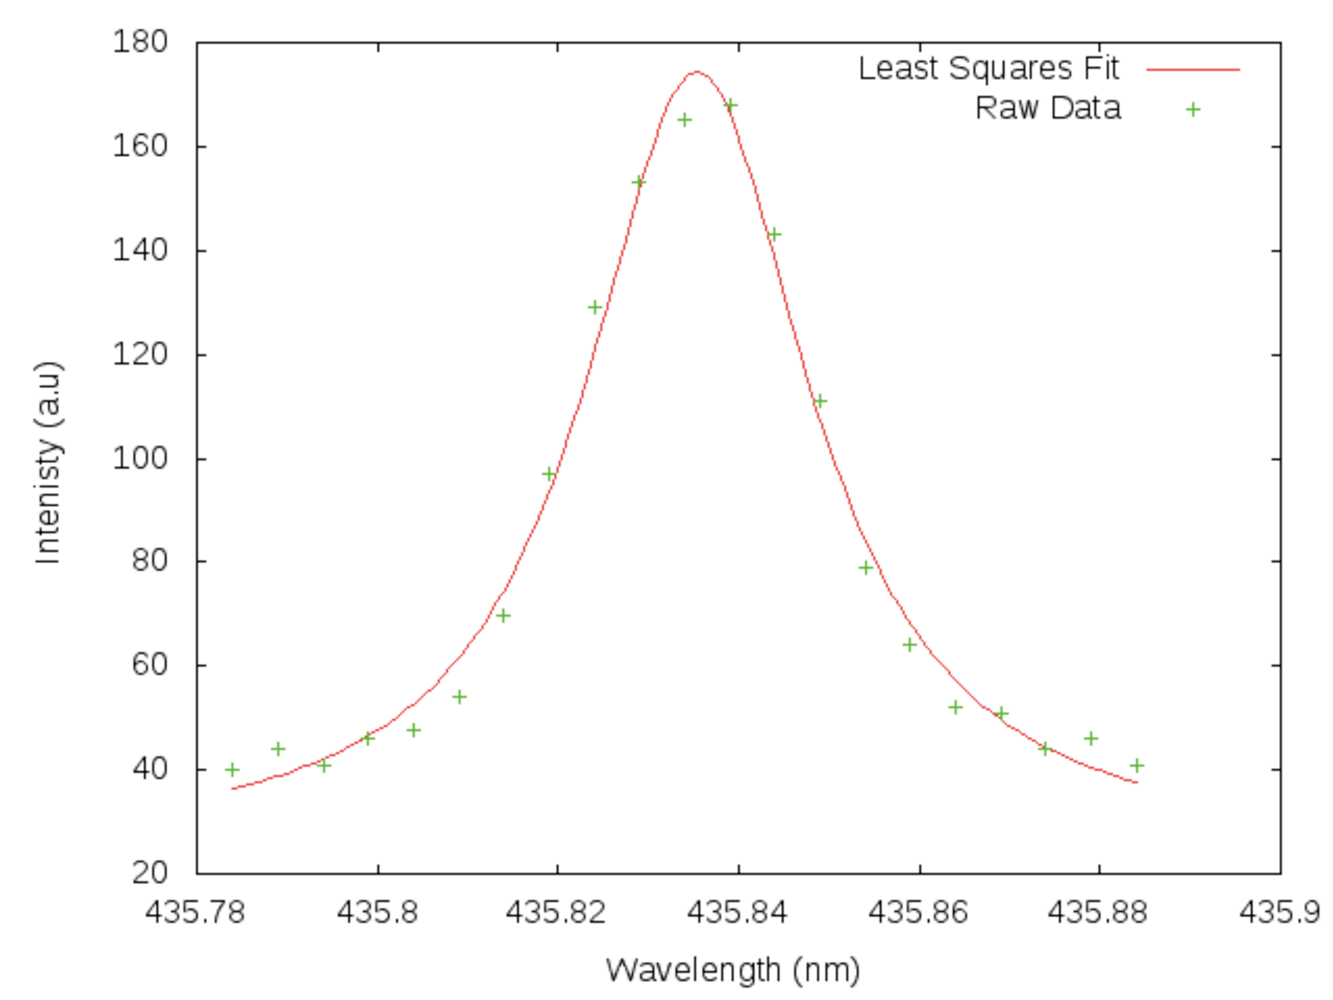
\includegraphics[width =120 mm, height = 70mm]{Ex_3_21.pdf}
\caption{A fit of fictional atomic excitation data using non-linear least squares.}
\label{fig:3.21}
\end{figure}
Using the algorithm developed above, the parameters were found to be the following
\begin{center}
Table 5:  Non-Linear Least Squares Parameters \\
\begin{tabular}{ | c | c |}
\hline
$I_0$ &  150.160615\\ \hline
$\lambda_0$ &  435.835389 \\ \hline
$\Gamma$ &0.030332   \\ \hline
$B$ &  24.307830\\ \hline
\end{tabular}
\end{center}
It is likely that this fictional data was intended to represent the excitation of the hydrogen atom, which has a characteristic emission at $435$ nm, which is quite close to the wavelength parameter obtained.
\section{Conclusions}
Throughout this lab, several different interpolation and fitting techniques were discussed.  Each has its own merits but they are all very versatile and incredibly valuable.  The Lagrange, Hermite, and Cubic Spline techniques were each applied to different types of Bessel functions and the applications of these functions to optical diffraction.  Additionally, two different matrix solving techniques were developed for use in the Cubic Spline and linear least squares fitting methods.  Several numerical approximations for the derivatives of a function were also presented and applied to a simple test function.  Finally, non-linear least squares fitting was used to model a set of fictional atomic excitation data.  These techniques were all successfully demonstrated and their value is quite apparent.


\pagebreak
\section{Code}
\subsection{Exercise 3.2}
\begin{verbatim}
#include <stdio.h>
#include <stdlib.h>
#include <math.h>

// Mitchell Miller
// PHYS 440 Lab 2
// Exc. 3.2 1/31/12
// Lagrange Interpolation

double lagrangeInterpolation(int numberPoints, double *positionMatrix, double *valueMatrix, double interpolationPoint){

	int counter1,counter2;
	double product,sum=0;

	for(counter1=0;counter1<numberPoints;counter1++){

		product = 1;
		for(counter2=0;counter2<numberPoints;counter2++){

			if(counter1!=counter2){

				//Calculate lambda
				product = product * ((interpolationPoint - positionMatrix[counter2]) / (positionMatrix[counter1] - positionMatrix[counter2]));
				//printf("prod = %lf\n",product);

			}
			
		}

		//Calcualte g(x)
		sum += product*valueMatrix[counter1];

	}

	printf("g(x) = %lf\n",sum);
	return sum;

}

int main(){

	int numberPoints = 21;
	int counter1;
	double positionMatrix[21] = {-5.,-4.5,-4.,-3.5,-3.,-2.5,-2.,-1.5,-1.,-0.5,0,0.5,1.,1.5,2.,2.5,3.,3.5,4.,4.5,5.};
	double valueMatrix[21] = {0.,0.,0.,0.,0.,0.,0.,0.00000000000000935918,000000000.206115,0.0000453979,0.5,0.999955,1.,1.,1.,1.,1.,1.,1.,1.};
	double pointValue;
	double calcPoint=-1.0;
	FILE *outfile;
	outfile = fopen("Ex_3.2.out.dat","w");

	//Calculate interpolation at points between -1 and 1
	for(counter1=0;counter1<200;counter1++){
		
		pointValue = lagrangeInterpolation(numberPoints,positionMatrix,valueMatrix,calcPoint);
		fprintf(outfile,"%lf\t%lf\n",calcPoint,pointValue);
		calcPoint = calcPoint + 0.01;
		printf("CalcPoint = %lf\n",calcPoint);

	}
	fclose(outfile);

}
\end{verbatim}
\subsection{Excersize 3.3}
\begin{verbatim}
#include <stdio.h>
#include <stdlib.h>
#include <math.h>

// Mitchell Miller
// PHYS 440 Lab 2
// Exc. 3.2 1/31/12
// Lagrange Interpolation

// I/I0 = (2*J0(x)/x)^2

// Interpolate the Airy pattern
// 10 Data points between 1 and 10
// http://keisan.casio.com/has10/SpecExec.cgi

double lagrangeInterpolation(int numberPoints, double *positionMatrix, double *valueMatrix, double interpolationPoint){

	int counter1,counter2;
	double product,sum=0;

	for(counter1=0;counter1<numberPoints;counter1++){

		product = 1;
		for(counter2=0;counter2<numberPoints;counter2++){

			if(counter1!=counter2){

				//Calculate lambda
				product = product * ((interpolationPoint - positionMatrix[counter2]) / (positionMatrix[counter1] - positionMatrix[counter2]));
				//printf("prod = %lf\n",product);

			}
			
		}

		//Calcualte g(x)
		sum += product*valueMatrix[counter1];

	}

	printf("g(x) = %lf\n",sum);
	return sum;

}

int main(){

	int numberPoints = 11;
	int counter1;
	double positionMatrix[11] = {0.1, 1.0,2.0,3.0,4.0,5.0,6.0,7.0,8.0,9.0,10.0};
	double valueMatrix[11] = {0.997503, 0.774578, 0.332612, 0.0510938, 0.00109043, 0.0171693, 0.008506, 0.00000179011, 0.00344089, 0.00297175, 0.0000755952};
	double pointValue;
	double calcPoint=0.0;
	FILE *outfile;
	FILE *outfileI;
	outfile = fopen("Ex_3.3.airy.dat","w");
	outfileI = fopen("airy.dat","w");

	//Calculate interpolation at points between -1 and 1
	for(counter1=0;counter1<100;counter1++){
		
		pointValue = lagrangeInterpolation(numberPoints,positionMatrix,valueMatrix,calcPoint);
		fprintf(outfile,"%lf\t%lf\n",calcPoint,pointValue);
		calcPoint = calcPoint + 0.1;
		printf("CalcPoint = %lf\n",calcPoint);

	}
	for(counter1=0;counter1<11;counter1++){
		
		fprintf(outfileI,"%lf\t%lf\n",positionMatrix[counter1],valueMatrix[counter1]);

	}
	fclose(outfile);

}
\\
#include <stdio.h>
#include <stdlib.h>
#include <math.h>

// Mitchell Miller
// PHYS 440 Lab 2
// Exc. 3.2 1/31/12
// Lagrange Interpolation

// Interpolate the J0 Bessel function using 3 points at a time
// 21 Data points between 0 and 10
// http://keisan.casio.com/has10/SpecExec.cgi

double lagrangeInterpolation(int numberPoints, double *positionMatrix, double *valueMatrix, double interpolationPoint){

	int counter1,counter2;
	double product,sum=0;

	for(counter1=0;counter1<numberPoints;counter1++){

		product = 1;
		for(counter2=0;counter2<numberPoints;counter2++){

			if(counter1!=counter2){

				//Calculate lambda
				product = product * ((interpolationPoint - positionMatrix[counter2]) / (positionMatrix[counter1] - positionMatrix[counter2]));
				//printf("prod = %lf\n",product);

			}
			
		}

		//Calcualte g(x)
		sum += product*valueMatrix[counter1];

	}

	printf("g(x) = %lf\n",sum);
	return sum;

}

int main(){

	int numberPoints = 21;
	int counter1;
	double positionMatrix[21] = {0.0,0.5,1.0,1.5,2.0,2.5,3.0,3.5,4.0,4.5,5.0,5.5,6.0,6.5,7.0,7.5,8.0,8.5,9.0,9.5,10.0};
	double valueMatrix[21] = {0,0.2422684577,0.4400505857,0.5579365079,0.5767248078,0.497094102,0.3390589585,0.1373775274,-0.06604332802,-0.2310604319,-0.3275791376,-0.3414382154,-0.2766838581,-0.1538413014,-0.0046828235,0.1352484276,0.2346363469,0.2731219637,0.2453117866,0.1612644308,0.04347274617};
	double pointValue;
	double calcPoint=0.0;
	FILE *outfile;
	outfile = fopen("Ex_3.3.j0.dat","w");

	//Calculate interpolation at points between -1 and 1
	for(counter1=0;counter1<100;counter1++){
		
		pointValue = lagrangeInterpolation(numberPoints,positionMatrix,valueMatrix,calcPoint);
		fprintf(outfile,"%lf\t%lf\n",calcPoint,pointValue);
		calcPoint = calcPoint + 0.1;
		printf("CalcPoint = %lf\n",calcPoint);

	}
	fclose(outfile);

}
\\
#include <stdio.h>
#include <stdlib.h>
#include <math.h>

// Mitchell Miller
// PHYS 440 Lab 2
// Exc. 3.2 1/31/12
// Lagrange Interpolation

// Interpolate the J0 Bessel function
// 21 Data points between 0 and 10
// http://keisan.casio.com/has10/SpecExec.cgi

double lagrangeInterpolation(int numberPoints, double *positionMatrix, double *valueMatrix, double interpolationPoint){

	int counter1,counter2;
	double product,sum=0;

	for(counter1=0;counter1<numberPoints;counter1++){

		product = 1;
		for(counter2=0;counter2<numberPoints;counter2++){

			if(counter1!=counter2){

				//Calculate lambda
				product = product * ((interpolationPoint - positionMatrix[counter2]) / (positionMatrix[counter1] - positionMatrix[counter2]));
				//printf("prod = %lf\n",product);

			}
			
		}

		//Calcualte g(x)
		sum += product*valueMatrix[counter1];

	}

	printf("g(x) = %lf\n",sum);
	return sum;

}

int main(){

	int numberPoints = 3;
	int counter1;
	double positionMatrix[3] = {2.0,2.5,3.0};
	double valueMatrix[3] = {0.2238907791,-0.04838377647,-0.2600519549};
	double pointValue;
	double calcPoint=1.0;
	FILE *outfile;
	outfile = fopen("Ex_3.3.j0.3point.dat","w");

	//Calculate interpolation at points between -1 and 1
	for(counter1=0;counter1<40;counter1++){
		
		pointValue = lagrangeInterpolation(numberPoints,positionMatrix,valueMatrix,calcPoint);
		fprintf(outfile,"%lf\t%lf\n",calcPoint,pointValue);
		calcPoint = calcPoint + 0.1;
		printf("CalcPoint = %lf\n",calcPoint);

	}
	fclose(outfile);

}
\\
#include <stdio.h>
#include <stdlib.h>
#include <math.h>

// Mitchell Miller
// PHYS 440 Lab 2
// Exc. 3.2 1/31/12
// Lagrange Interpolation

// Interpolate the J0 Bessel function
// 21 Data points between 0 and 10
// http://keisan.casio.com/has10/SpecExec.cgi

double lagrangeInterpolation(int numberPoints, double *positionMatrix, double *valueMatrix, double interpolationPoint){

	int counter1,counter2;
	double product,sum=0;

	for(counter1=0;counter1<numberPoints;counter1++){

		product = 1;
		for(counter2=0;counter2<numberPoints;counter2++){

			if(counter1!=counter2){

				//Calculate lambda
				product = product * ((interpolationPoint - positionMatrix[counter2]) / (positionMatrix[counter1] - positionMatrix[counter2]));
				//printf("prod = %lf\n",product);

			}
			
		}

		//Calcualte g(x)
		sum += product*valueMatrix[counter1];

	}

	printf("g(x) = %lf\n",sum);
	return sum;

}

int main(){

	int numberPoints = 21;
	int counter1;
	double positionMatrix[21] = {0.0,0.5,1.0,1.5,2.0,2.5,3.0,3.5,4.0,4.5,5.0,5.5,6.0,6.5,7.0,7.5,8.0,8.5,9.0,9.5,10.0};
	double valueMatrix[21] = {1,0.9384698072,0.7651976866,0.5118276717,0.2238907791,-0.04838377647,-0.2600519549,-0.38012774,-0.3971498099,-0.320542509,-0.1775967713,-0.0068438694,0.1506452573,0.260094606,0.3000792705,0.2663396579,0.1716508071,0.0419392518,-0.0903336112,-0.1939287477,-0.2459357645};
	double pointValue;
	double calcPoint=0.0;
	FILE *outfile;
	outfile = fopen("Ex_3.3.j0.dat","w");

	//Calculate interpolation at points between -1 and 1
	for(counter1=0;counter1<100;counter1++){
		
		pointValue = lagrangeInterpolation(numberPoints,positionMatrix,valueMatrix,calcPoint);
		fprintf(outfile,"%lf\t%lf\n",calcPoint,pointValue);
		calcPoint = calcPoint + 0.1;
		printf("CalcPoint = %lf\n",calcPoint);

	}
	fclose(outfile);

}
\\
#include <stdio.h>
#include <stdlib.h>
#include <math.h>

// Mitchell Miller
// PHYS 440 Lab 2
// Exc. 3.2 1/31/12
// Lagrange Interpolation

// Interpolate the J1 Bessel function
// 21 Data points between 0 and 10
// http://keisan.casio.com/has10/SpecExec.cgi

double lagrangeInterpolation(int numberPoints, double *positionMatrix, double *valueMatrix, double interpolationPoint){

	int counter1,counter2;
	double product,sum=0;

	for(counter1=0;counter1<numberPoints;counter1++){

		product = 1;
		for(counter2=0;counter2<numberPoints;counter2++){

			if(counter1!=counter2){

				//Calculate lambda
				product = product * ((interpolationPoint - positionMatrix[counter2]) / (positionMatrix[counter1] - positionMatrix[counter2]));
				//printf("prod = %lf\n",product);

			}
			
		}

		//Calcualte g(x)
		sum += product*valueMatrix[counter1];

	}

	printf("g(x) = %lf\n",sum);
	return sum;

}

int main(){

	int numberPoints = 21;
	int counter1;
	double positionMatrix[21] = {0.0,0.5,1.0,1.5,2.0,2.5,3.0,3.5,4.0,4.5,5.0,5.5,6.0,6.5,7.0,7.5,8.0,8.5,9.0,9.5,10.0};
	double valueMatrix[21] = {0,0.2422684577,0.4400505857,0.5579365079,0.5767248078,0.497094102,0.3390589585,0.1373775274,-0.06604332802,-0.2310604319,-0.3275791376,-0.3414382154,-0.2766838581,-0.1538413014,-0.0046828235,0.1352484276,0.2346363469,0.2731219637,0.2453117866,0.1612644308,0.04347274617};
	double pointValue;
	double calcPoint=0.0;
	FILE *outfile;
	outfile = fopen("Ex_3.3.j1.dat","w");

	//Calculate interpolation at points between -1 and 1
	for(counter1=0;counter1<100;counter1++){
		
		pointValue = lagrangeInterpolation(numberPoints,positionMatrix,valueMatrix,calcPoint);
		fprintf(outfile,"%lf\t%lf\n",calcPoint,pointValue);
		calcPoint = calcPoint + 0.1;
		printf("CalcPoint = %lf\n",calcPoint);

	}
	fclose(outfile);

}
\end{verbatim}
\subsection{Exercise 3.4}
\begin{verbatim}
#include <stdio.h>
#include <stdlib.h>
#include <math.h>

// Mitchell Miller
// PHYS 440 Lab 2
// Exc. 3.2 2/11/12
// Hermite Interpolation

// I/I0 = (2*J0(x)/x)^2

// Interpolate the Airy pattern
// 10 Data points between 1 and 10
// http://keisan.casio.com/has10/SpecExec.cgi

double hermiteInterpolation(int numberPoints, double *positionMatrix, double *valueMatrix, double *derivativeMatrix, double interpolationPoint){

	int counter1,counter2;
	double product,sum=0,poly=0;
	double hj, hjp;

	for(counter1=0;counter1<numberPoints;counter1++){

		product = 1;
		sum = 0;
		for(counter2=0;counter2<numberPoints;counter2++){

			if(counter1!=counter2){

				//Calculate lambda
				product = product * ((interpolationPoint - positionMatrix[counter2]) / (positionMatrix[counter1] - positionMatrix[counter2]));
				sum = sum + 1./(positionMatrix[counter1] - positionMatrix[counter2]);

			}
			
		}

		//Calcualte g(x)
		hj = (1. - 2.*(interpolationPoint - positionMatrix[counter1]) * sum) * product * product;
		hjp = (interpolationPoint - positionMatrix[counter1]) * product * product;
		poly = poly + hj*valueMatrix[counter1] + hjp*derivativeMatrix[counter1];

	}

	printf("g(x) = %lf\n",poly);
	return poly;

}

int main(){

	int numberPoints = 11;
	int counter1;
	double positionMatrix[11] = {0.1,1.0,2.0,3.0,4.0,5.0,6.0,7.0,8.0,9.0,10.0};
	double valueMatrix[11] = {0.997503, 0.774578, 0.332612, 0.0510938, 0.00109043, 0.0171693, 0.008506, 0.00000179011, 0.00344089, 0.00297175, 0.0000755952};
	double derivativeMatrix[11] = {-0.0498959,-0.404507,-0.406976,-0.146501,0.0120241,0.0048812,-0.0149331,-0.000230446,0.003314,-0.00350941,-0.000885558};
	double pointValue;
	double calcPoint=0.0;
	FILE *outfile;
	outfile = fopen("Ex_3.4.airy.dat","w");

	//Calculate interpolation at points between -1 and 1
	for(counter1=0;counter1<100;counter1++){
		
		printf("CalcPoint = %lf\n",calcPoint);
		pointValue = hermiteInterpolation(numberPoints,positionMatrix,valueMatrix,derivativeMatrix,calcPoint);
		fprintf(outfile,"%lf\t%lf\n",calcPoint,pointValue);
		calcPoint = calcPoint + 0.1;

	}
	fclose(outfile);

}
\\
#include <stdio.h>
#include <stdlib.h>
#include <math.h>

// Mitchell Miller
// PHYS 440 Lab 2
// Exc. 3.2 2/11/12
// Hermite Interpolation

// Interpolate the J0 Bessel function
// 11 Data points between 0 and 10
// http://keisan.casio.com/has10/SpecExec.cgi

double hermiteInterpolation(int numberPoints, double *positionMatrix, double *valueMatrix, double *derivativeMatrix, double interpolationPoint){

	int counter1,counter2;
	double product,sum=0,poly=0;
	double hj, hjp;

	for(counter1=0;counter1<numberPoints;counter1++){

		product = 1;
		sum = 0;
		for(counter2=0;counter2<numberPoints;counter2++){

			if(counter1!=counter2){

				//Calculate lambda
				product = product * ((interpolationPoint - positionMatrix[counter2]) / (positionMatrix[counter1] - positionMatrix[counter2]));
				sum = sum + 1./(positionMatrix[counter1] - positionMatrix[counter2]);

			}
			
		}

		//Calcualte g(x)
		hj = (1. - 2.*(interpolationPoint - positionMatrix[counter1]) * sum) * product * product;
		hjp = (interpolationPoint - positionMatrix[counter1]) * product * product;
		poly = poly + hj*valueMatrix[counter1] + hjp*derivativeMatrix[counter1];

	}

	printf("g(x) = %lf\n",poly);
	return poly;

}

int main(){

	int numberPoints = 11;
	int counter1;
	double positionMatrix[11] = {0.0,1.0,2.0,3.0,4.0,5.0,6.0,7.0,8.0,9.0,10.0};
	double valueMatrix[11] = {1.,0.7651976866,0.2238907791,-0.2600519549,-0.3971498099,-0.1775967713,0.1506452573,0.3000792705,0.1716508071,-0.0903336112,-0.2459357645};
	double derivativeMatrix[11] = {0.0, -0.4400505857, -0.5767248078, -0.3390589585, 0.0660433280, 0.3275791376, 0.2766838581, 0.0046828235, -0.2346363469, -0.2453117866, -0.0434727462};
	double pointValue;
	double calcPoint=0.0;
	FILE *outfile;
	outfile = fopen("Ex_3.4.j0.dat","w");

	//Calculate interpolation at points between -1 and 1
	for(counter1=0;counter1<100;counter1++){
		
		printf("CalcPoint = %lf\n",calcPoint);
		pointValue = hermiteInterpolation(numberPoints,positionMatrix,valueMatrix,derivativeMatrix,calcPoint);
		fprintf(outfile,"%lf\t%lf\n",calcPoint,pointValue);
		calcPoint = calcPoint + 0.1;

	}
	fclose(outfile);

}
\\
#include <stdio.h>
#include <stdlib.h>
#include <math.h>

// Mitchell Miller
// PHYS 440 Lab 2
// Exc. 3.2 2/11/12
// Hermite Interpolation

// J1' = (J0 - J2) / 2

// Interpolate the J1 Bessel function
// 11 Data points between 0 and 10
// http://keisan.casio.com/has10/SpecExec.cgi

double hermiteInterpolation(int numberPoints, double *positionMatrix, double *valueMatrix, double *derivativeMatrix, double interpolationPoint){

	int counter1,counter2;
	double product,sum=0,poly=0;
	double hj, hjp;

	for(counter1=0;counter1<numberPoints;counter1++){

		product = 1;
		sum = 0;
		for(counter2=0;counter2<numberPoints;counter2++){

			if(counter1!=counter2){

				//Calculate lambda
				product = product * ((interpolationPoint - positionMatrix[counter2]) / (positionMatrix[counter1] - positionMatrix[counter2]));
				sum = sum + 1./(positionMatrix[counter1] - positionMatrix[counter2]);

			}
			
		}

		//Calcualte g(x)
		hj = (1. - 2.*(interpolationPoint - positionMatrix[counter1]) * sum) * product * product;
		hjp = (interpolationPoint - positionMatrix[counter1]) * product * product;
		poly = poly + hj*valueMatrix[counter1] + hjp*derivativeMatrix[counter1];

	}

	printf("g(x) = %lf\n",poly);
	return poly;

}

int main(){

	int numberPoints = 11;
	int counter1;
	double positionMatrix[11] = {0.0,1.0,2.0,3.0,4.0,5.0,6.0,7.0,8.0,9.0,10.0};
	double valueMatrix[11] = {0.,0.4400505857,0.5767248078,0.3390589585,-0.06604332802,-0.3275791376,-0.2766838581,-0.0046828235,0.2346363469,0.2453117866,0.04347274617};
	double derivativeMatrix[11] = {0.5, 0.325147, -0.0644716, -0.373072, -0.380639, -0.112081, 0.196759, 0.300748, 0.142321, -0.11759, -0.250283};
	double pointValue;
	double calcPoint=0.0;
	FILE *outfile;
	outfile = fopen("Ex_3.4.j1.dat","w");

	//Calculate interpolation at points between -1 and 1
	for(counter1=0;counter1<100;counter1++){
		
		printf("CalcPoint = %lf\n",calcPoint);
		pointValue = hermiteInterpolation(numberPoints,positionMatrix,valueMatrix,derivativeMatrix,calcPoint);
		fprintf(outfile,"%lf\t%lf\n",calcPoint,pointValue);
		calcPoint = calcPoint + 0.1;

	}
	fclose(outfile);

}
\end{verbatim}
\subsection{Exercise 3.5}
\begin{verbatim}
#include <stdio.h>
#include <stdlib.h>
#include <math.h>

// Mitchell Miller
// PHYS 440 Lab 2
// Exc. 3.5 2/11/12
// Trisolve Method

int main(){

	int counter;
	int diagLength = 5;
	double aMat[5] = {-1.0,-1.0,-1.0,-1.0,-1.0};
	double bMat[5] = {2.,2.,2.,2.,2.};
	double cMat[5] = {-1.0,-1.0,-1.0,-1.0,-1.0};
	double rMat[5] = {0.,1.,2.,3.,4.};
	double rhoMat[5] = {0.,0.,0.,0.,0.};
	double betaMat[5] = {0.,0.,0.,0.,0.};

	betaMat[0] = bMat[0];
	rhoMat[0] = rMat[0];

	for(counter = 1; counter < diagLength; counter++){

		betaMat[counter] = bMat[counter] - (aMat[counter] * cMat[counter-1])/betaMat[counter-1];
		rhoMat[counter] = rMat[counter] - (aMat[counter] * rhoMat[counter-1])/betaMat[counter-1];

	}

	rhoMat[diagLength-1] = rhoMat[diagLength-1] / betaMat[diagLength-1];

	for(counter = 1; counter < diagLength; counter++){

		rhoMat[diagLength-1-counter] = (rhoMat[diagLength-1-counter] - cMat[diagLength-1-counter] * rhoMat[diagLength-counter]) / betaMat[diagLength-1-counter];

	}

	for(counter = 0; counter < diagLength; counter++){

		printf("X_%i = %lf\n", counter, rhoMat[counter]);

	}

}
\end{verbatim}
\subsection{Exercise 3.6}
\begin{verbatim}
#include <stdio.h>
#include <stdlib.h>
#include <math.h>

// Mitchell Miller
// PHYS 440 Lab 2
// Exc. 3.6 2/11/12
// Cubic Spline Fitting

// NOTE THAT N SHOULD BE THE INDEX VALUE, NOT THE NUMBER OF POINTS

double spline(double xValue, double *x, double *f, double *second, int N){

	int counter = 0;
	double sp1,sp2,sp3,sp4,spline;	
	
	// Check bounds
	if(xValue < x[0]){

		printf("X Value is less than x[0] in spline");
		exit(1);
	
	}
	if(xValue > x[N]){

		printf("X Value is greater than x[0] in spline");
		exit(1);

	}


	// Find interval containing xValue
	while(xValue > x[counter+1]){

		counter = counter + 1;

	}

	// Begin interpolation
	sp1 = (xValue - x[counter]) * ((f[counter+1] - f[counter]) / (x[counter+1] - x[counter]));
	sp2 = (xValue - x[counter]) * (x[counter+1] - x[counter]) * (second[counter+1]/6.0 + second[counter]/3.0);
	sp3 = 0.5 * second[counter] * (xValue - x[counter]) * (xValue - x[counter]);
	sp4 = ((second[counter+1] - second[counter]) * (xValue - x[counter]) * (xValue - x[counter]) * (xValue - x[counter]) / (6.0 * (x[counter+1] - x[counter])));
	spline = f[counter] + sp1 - sp2 + sp3 + sp4;

	return spline;

}

void *splineInit(double *x, double *f, double *second, double fp1, double fpn, int N){

	int counter = 0;
	double beta[11] = { 0 };
	double b0,r0,bj,rj,aj,c;
	
	b0 = 2.0 * (x[1] - x[0]);
	beta[0] = b0;
	r0 = 6.0 * ((f[1] - f[0]) / (x[1] - x[0]) - fp1);

	for(counter=1;counter<=N;counter++){

		if(counter == N){

			bj = 2.0 * (x[N] - x[N-1]);
			rj = -6.0 * ((f[N] - f[N-1]) / (x[N] - x[N-1]) - fpn);

		}
		else{
			
			bj = 2.0 * (x[counter+1] - x[counter-1]);
			rj = 6.0 * ((f[counter+1] - f[counter]) / (x[counter+1] - x[counter]) - (f[counter] - f[counter-1]) / (x[counter] - x[counter-1]));

		}

		aj = x[counter] - x[counter-1];
		c = aj;
		beta[counter] = bj - aj * c / beta[counter-1];
		second[counter] = rj - aj * second[counter-1] / beta[counter-1];

		if(beta[counter] == 0.){
	
			printf("Zero element in diagonal of splineinit");
			exit(1);

		}

	}

	second[N] = second[N]/beta[N];

	for(counter=0;counter<N;counter++){

		c = x[N-counter+1] - x[N-counter];
		second[N-counter] = (second[N-counter] - c * second[N-counter+1]) / beta[N-counter];

	}

}

int main(){

	int numberOfPoints = 10;
	int counter = 0;
	double *secondDeriv = malloc(11*sizeof(double));
	double positionMatrix[11] = {0.0,1.0,2.0,3.0,4.0,5.0,6.0,7.0,8.0,9.0,10.0};
	double valueMatrix[11] = {0.,0.4400505857,0.5767248078,0.3390589585,-0.06604332802,-0.3275791376,-0.2766838581,-0.0046828235,0.2346363469,0.2453117866,0.04347274617};
	double valueDeriv1 = 0.5;
	double valueDerivN = -0.250283;
	double interpPoint = 0.0;
	double interpValue;
	FILE *outfile;
	outfile = fopen("Ex_3.6.dat","w");
	
	splineInit(positionMatrix,valueMatrix,secondDeriv,valueDeriv1,valueDerivN,numberOfPoints);

	/*for(counter=0;counter<11;counter++){
		printf("g''(%lf) = %ls\n",counter,secondDeriv[counter]);
	}*/

	for(counter=0;counter<100;counter++){

		interpValue = spline(interpPoint,positionMatrix,valueMatrix,secondDeriv,numberOfPoints);
		printf("g(%lf) = %lf\n", interpPoint, interpValue);
		fprintf(outfile,"%lf\t%lf\n",interpPoint,interpValue);
		interpPoint = interpPoint + 0.1;

	}

}
\end{verbatim}
\subsection{Exercise 3.13}
\begin{verbatim}
#include <stdio.h>
#include <stdlib.h>
#include <math.h>
#define e 2.71828182845

// Mitchell Miller
// PHYS 440 Lab 2
// Exc. 3.13 2/17/12

double function(double x){
	//Specify your desired function
	return(x*pow(e,x));
	//return(cos(x));
}

double forwardDiff(double xValue, double stepSize){
	double differentiatedValue;

	differentiatedValue = (function(xValue+stepSize) - function(xValue)) / stepSize;
	return(differentiatedValue);

}

double centralDiff(double xValue, double stepSize){
	double differentiatedValue;

	differentiatedValue = (function(xValue+stepSize)-function(xValue-stepSize)) / (2.*stepSize);
	return(differentiatedValue);

}

double extrapolatedDiff(double xValue, double stepSize){
	double differentiatedValue;

	differentiatedValue = (function(xValue) - function(xValue-stepSize)) / stepSize;
	return(differentiatedValue);

}

double forwardSecDiff(double xValue, double stepSize){

	double differentiatedValue;

	differentiatedValue = ((function(xValue) - 2.0*function(xValue+stepSize) + function(xValue+2.0*stepSize)) / (stepSize * stepSize));

	return(differentiatedValue);

}

double centralSecDiff(double xValue, double stepSize){

	double differentiatedValue;

	differentiatedValue = ((function(xValue+stepSize) - 2.0*function(xValue) + function(xValue-stepSize)) / (stepSize * stepSize));

	return(differentiatedValue);

}

int main(){
	//Initialize variables
	double stepSize=0.5;
	int counter;
	double forSolution,cenSolution,extSolution,for2Solution,cen2Solution;
	double forError,cenError,extError,for2Error,cen2Error;
	double firstDeriv = 22.1671682967920;
	double secondDeriv = 29.5562243957226;
	FILE *outfile;
	outfile=fopen("Ex_3.13.error.dat","w");
	fprintf(outfile,"#N\teps_F\teps_C\teps_E\teps_F2\teps_C2\n");

	//Calculate values
	for(counter=0;counter<45;counter++){
		forSolution = forwardDiff(2.0,stepSize);
		cenSolution = centralDiff(2.0,stepSize);
		extSolution = extrapolatedDiff(2.0,stepSize);
		for2Solution = forwardSecDiff(2.0,stepSize);
		cen2Solution = centralSecDiff(2.0,stepSize);

		//Calculate error
		forError = fabs((firstDeriv-forSolution) / firstDeriv);
		cenError = fabs((firstDeriv-cenSolution) / firstDeriv);
		extError = fabs((firstDeriv-extSolution) / firstDeriv);
		for2Error = fabs((secondDeriv-for2Solution) / secondDeriv);
		cen2Error = fabs((secondDeriv-cen2Solution) / secondDeriv);
		
		//Print results
		printf("h = %lf\n", stepSize);
		printf("Forward Error = %e\n", forError);
		printf("Central Error = %e\n", cenError);
		printf("Extrapolated Error = %e\n", extError);
		printf("Forward 2nd Deriv Error = %e\n", for2Error);
		printf("Central 2nd Deriv Error = %e\n", cen2Error);
		fprintf(outfile,"%lf\t%.20lf\t%.20lf\t%.20lf\t%.20lf\t%.20lf\n",stepSize,forError,cenError,extError,for2Error,cen2Error);
		stepSize = stepSize - 0.01;
	}

	fclose(outfile);

}
\\
#include <stdio.h>
#include <stdlib.h>
#include <math.h>
#define e 2.71828182845

// Mitchell Miller
// PHYS 440 Lab 2
// Exc. 3.13 2/17/12
// Richardson Extrapolation

double function(double x){
	//Specify your desired function
	return(x*pow(e,x));
	//return(cos(x));
}

double centralDiff(double xValue, double stepSize){
	double differentiatedValue;

	differentiatedValue = (function(xValue+stepSize)-function(xValue-stepSize)) / (2.0*stepSize);
	return(differentiatedValue);

}

double richardson(int i, double Dih, double Dihh){

	double Dii;

	Dii = (pow(2.0,2.0*i)*Dih - Dihh) / (pow(2.0,2.0*i) - 1);

	return(Dii);

}

int main(){

	double D[4][4] = {{0,0,0,0},{0,0,0,0},{0,0,0,0},{0,0,0,0}};
	double stepSize = 0.4;
	int counter = 1;
	int counter2;
	FILE *outfile;
	outfile = fopen("Ex_3.13.richardson.dat","w");
	fprintf(outfile,"h & $D_1$ & $D_2$ & $D_3$ & $D_4$ \\\\ \hline\n");

	// Build first column from central difference method
	for(counter=0;counter<4;counter++){

		stepSize = 0.4 / pow(2,counter);
		D[counter][0] = centralDiff(2.0,stepSize);
	
	}


	// Build table from Richardson extr.
	for(counter2=1;counter2<4;counter2++){

		for(counter=counter2-1;counter<4;counter++){

			D[counter][counter2] = richardson(counter2, D[counter][counter2-1], D[counter-1][counter2-1]);

		}

	}

	for(counter2=0;counter2<4;counter2++){

		fprintf(outfile,"%.3lf",0.4/pow(2,counter2));
		for(counter=0;counter<4;counter++){

			//printf("D_%i(%lf) = %lf\n",counter2+1,0.4/(pow(2,counter)),D[counter][counter2]);
			if(D[counter2][counter]<24 && D[counter2][counter]>21){

				fprintf(outfile," & %lf", D[counter2][counter]);
			
			}
			else{

				fprintf(outfile," & ");

			}

		}

		fprintf(outfile," \\\\ \hline\n");

	}

}
\end{verbatim}
\subsection{Exercise 3.17}
\begin{verbatim}
#include <stdio.h>
#include <stdlib.h>
#include <math.h>

// Mitchell Miller
// PHYS 440 Lab 2
// Exc. 3.17 2/18/12
// LU Solve Method

// n is the number of index points, not number of points

double *luSolve(double **a, double *x, double *b, double det, int ndim, int n){

	int order[10],i,j,k,imax,itemp;
	double scale[10],max,sum,temp;

	det = 1.0;

	for(i=0;i<n;i++){

		order[i] = i;
		max = 0.;

		for(j=0;j<n;j++){

			if(fabs(a[i][j])>max){

				max = fabs(a[i][j]);

			}

		}

		scale[i] = 1.0 / max;

	}

	for(k=0;k<n-1;k++){

		if(k!=0){

			for(i=k;i<n;i++){

				sum = a[i][k];

				for(j=0;j<=k-1;j++){

					sum = sum - a[i][j]*a[j][k];

				}

				a[i][k] = sum;

			}

		}

		max = 0;

		for(i=k;i<n;i++){

			if(scale[i]*a[i][k] >= max){

				max = scale[i]*a[i][k];
				imax = i;

			}

		}

		if(imax!=k){

			det = -det;

			for(j=1;j<n;j++){

				temp = a[imax][j];
				a[imax][j] = a[k][j];
				a[k][j] = temp;

			}

			temp = scale[imax];
			scale[imax] = scale[k];
			scale[k] = temp;

			itemp = order[imax];
			order[imax] = order[k];
			order[k] = itemp;

		}

		det = det*a[k][k];

		if(k==0){

			for(j=1;j<n;j++){

				a[0][j] = a[0][j] / a[0][0];

			}

		}
		else{

			for(j=k+1;j<n;j++){

				sum = a[k][j];
		
				for(i=0;i<=k-1;i++){

					sum = sum - a[k][i]*a[i][j];
			
				}

				a[k][j] = sum / a[k][k];

			}

		}

	}

	sum = a[n-1][n-1];
	for(j=0;j<n-1;j++){

		sum = sum - a[n-1][j]*a[j][n-1];

	}
	a[n-1][n-1] = sum;
	det = det*a[n-1][n-1];


	// Begin solution


	for(i=0;i<n;i++){

		x[i] = b[order[i]];

	}

	x[0] = x[0] / a[0][0];

	for(i=1;i<n;i++){

		sum = x[i];

		for(k=0;k<=i-1;k++){

			sum = sum - a[i][k]*x[k];

		}

		x[i] = sum / a[i][i];

	}

	for(i=1;i<n;i++){

		sum = x[n-1-i];

		for(k=n-1-i+1;k<n;k++){

			sum = sum - a[n-1-i][k] * x[k];

		}

		x[n-1-i] = sum;

	}

}

int main(){

	double** a;
	int i;
	a = (double**) malloc(5*sizeof(double*));
	for(i=0;i<5;i++){
		a[i] = (double*) malloc(5*sizeof(double));
	}
	double *b = malloc(5*sizeof(double));
	double *x = malloc(5*sizeof(double));
	double det;

	a[0][0] = 2.0;
	a[4][4] = 2.0;
	
	for(i=1;i<5;i++){

		a[i][i] = 2.0;
		a[i-1][i] = -1.0;
		a[i][i-1] = -1.0;

	}

	b[0] = 0.0;
	b[1] = 1.0;
	b[2] = 2.0;
	b[3] = 3.0;
	b[4] = 4.0;

	luSolve(a,x,b,det,5,5.0);

	for(i=0;i<5;i++){

		printf("X[%i] = %lf\n",i,x[i]);

	}

}
\end{verbatim}
\subsection{Exercise 3.20}
\begin{verbatim}
#include <stdio.h>
#include <stdlib.h>
#include <math.h>

// Mitchell Miller
// PHYS 440 Lab 2
// Exc. 3.20 2/18/12
// Least Squares Fitting

void *luSolve(double **a, double *x, double *b, int n){

	int order[15],i,j,k,imax,itemp;
	double scale[15],max,sum,temp,det;

	det = 1.0;

	for(i=0;i<n;i++){

		order[i] = i;
		max = 0.;

		for(j=0;j<n;j++){

			if(fabs(a[i][j])>max){

				max = fabs(a[i][j]);

			}

		}

		scale[i] = 1.0 / max;

	}

	for(k=0;k<n-1;k++){

		if(k!=0){

			for(i=k;i<n;i++){

				sum = a[i][k];

				for(j=0;j<=k-1;j++){

					sum = sum - a[i][j]*a[j][k];

				}

				a[i][k] = sum;

			}

		}

		max = 0;

		for(i=k;i<n;i++){

			if(scale[i]*a[i][k] >= max){

				max = scale[i]*a[i][k];
				imax = i;

			}

		}

		if(imax!=k){

			det = -det;

			for(j=0;j<n;j++){

				temp = a[imax][j];
				a[imax][j] = a[k][j];
				a[k][j] = temp;

			}

			temp = scale[imax];
			scale[imax] = scale[k];
			scale[k] = temp;

			itemp = order[imax];
			order[imax] = order[k];
			order[k] = itemp;

		}

		det = det*a[k][k];

		if(k==0){

			for(j=1;j<n;j++){

				a[0][j] = a[0][j] / a[0][0];

			}

		}
		else{

			for(j=k+1;j<n;j++){

				sum = a[k][j];
		
				for(i=0;i<=k-1;i++){

					sum = sum - a[k][i]*a[i][j];
			
				}

				a[k][j] = sum / a[k][k];

			}

		}

	}

	sum = a[n-1][n-1];
	for(j=0;j<n-1;j++){

		sum = sum - a[n-1][j]*a[j][n-1];

	}
	a[n-1][n-1] = sum;
	det = det*a[n-1][n-1];


	// Begin solution


	for(i=0;i<n;i++){

		x[i] = b[order[i]];

	}

	x[0] = x[0] / a[0][0];

	for(i=1;i<n;i++){

		sum = x[i];

		for(k=0;k<=i-1;k++){

			sum = sum - a[i][k]*x[k];

		}

		x[i] = sum / a[i][i];

	}

	for(i=1;i<n;i++){

		sum = x[n-1-i];

		for(k=n-1-i+1;k<n;k++){

			sum = sum - a[n-1-i][k] * x[k];

		}

		x[n-1-i] = sum;

	}

}

int main(){

	int N=11;
	double** a;
	int i;
	a = (double**) malloc(3*sizeof(double*));
	for(i=0;i<3;i++){
		a[i] = (double*) malloc(3*sizeof(double));
	}
	double *b = malloc(3*sizeof(double));
	double *x = malloc(3*sizeof(double));

	double positionMatrix[11] = {0.,0.1,0.2,0.3,0.4,0.5,0.6,0.7,0.8,0.9,1.0};
	double valueMatrix[11] = {1.67203,1.79792,2.37791,2.66408,2.11245,2.43969,1.88843,1.59447,1.79634,1.07810,0.21066};
	FILE *outfile;
	outfile = fopen("Ex_3.20.dat","w");
	double temp=0;

	a[0][0]=11.;
	a[1][0]=5.5;
	a[0][1]=5.5;
	a[0][2]=3.85;
	a[2][0]=3.85;
	a[1][1]=3.85;
	a[1][2]=3.025;
	a[2][1]=3.025;
	a[2][2]=2.5333;

	b[0]=19.6321;
	b[1]=8.38663;
	b[2]=4.99548;

	/*
	// Fill in A matrix
	a[0][0]=11.;
	for(i=0;i<N;i++){

		temp = temp + positionMatrix[i];

	}
	a[0][1]=temp;
	a[1][0]=temp;
	temp=0;
	for(i=0;i<N;i++){

		temp = temp + positionMatrix[i]*positionMatrix[i];

	}
	a[0][2]=temp;
	a[1][1]=temp;
	a[2][0]=temp;
	temp=0;
	for(i=0;i<N;i++){

		temp = temp + positionMatrix[i]*positionMatrix[i]*positionMatrix[i];

	}
	a[1][2]=temp;
	a[2][1]=temp;
	temp=0;
	for(i=0;i<N;i++){

		temp = temp + positionMatrix[i]*positionMatrix[i]*positionMatrix[i]*positionMatrix[i];

	}
	a[2][2]=temp;
	temp=0;

	// Fill in B matrix
	for(i=0;i<N;i++){

		temp = temp + valueMatrix[i];

	}
	b[0] = temp;
	temp=0;
	for(i=0;i<N;i++){

		temp = temp + positionMatrix[i]*valueMatrix[i];

	}
	b[1]=temp;
	temp=0;
	for(i=0;i<N;i++){

		temp = temp + positionMatrix[i]*positionMatrix[i]*valueMatrix[i];

	}
	b[2]=temp;*/

	// Solve normal equations
	luSolve(a,x,b,3);

	for(i=0;i<3;i++){

		printf("C_%i = %lf\n",i,x[i]);

	}

	for(i=0;i<11;i++){

		fprintf(outfile,"%lf\t%lf\n",positionMatrix[i],valueMatrix[i]);

	}

}
\end{verbatim}
\subsection{Exercise 3.21}
\begin{verbatim}
#include <stdio.h>
#include <stdlib.h>
#include <math.h>

// Mitchell Miller
// PHYS 440 Lab 2
// Exc. 3.21 2/18/12
// Non-Linear Least Squares Fitting

void *init(double *a, double *h){

	int max=6;
	int m=4;

	if(m>max){

		printf("Dimensional error in init\n");
		exit(1);

	}

	a[0] = 435.84;
	a[1] = 0.03;
	a[2] = 120.;
	a[3] = 2.0;

	h[0] = 0.01;
	h[1] = 0.005;
	h[2] = 4.0;
	h[3] = 2.0;

}
/*
double sum(double *array, int size){

	int i;
	double sumA=0;
	for(i=0;i<size;i++){

		sumA = sumA + array[i];

	}
	return(sumA);

}*/

double sum(double *a){

	double x[21],y[21];
	double tc,lambda,lambdaO,baseline;
	double intensity,gamma;
	double sumA;
	int i;

	x[0] = 435.784;
	x[1] = 435.789;
	x[2] = 435.794;
	x[3] = 435.799;
	x[4] = 435.804;
	x[5] = 435.809;
	x[6] = 435.814;
	x[7] = 435.819;
	x[8] = 435.824;
	x[9] = 435.829;
	x[10] = 435.834;
	x[11] = 435.839;
	x[12] = 435.844;
	x[13] = 435.849;
	x[14] = 435.854;
	x[15] = 435.859;
	x[16] = 435.864;
	x[17] = 435.869;
	x[18] = 435.874;
	x[19] = 435.879;
	x[20] = 435.884;
	
	y[0] = 40.0;
	y[1] = 44.0;
	y[2] = 41.0;
	y[3] = 46.0;
	y[4] = 47.5;
	y[5] = 54.0;
	y[6] = 69.7;
	y[7] = 97.0;
	y[8] = 129.0;
	y[9] = 153.0;
	y[10] = 165.0;
	y[11] = 168.0;
	y[12] = 143.0;
	y[13] = 111.0;
	y[14] = 79.0;
	y[15] = 64.0;
	y[16] = 52.0;
	y[17] = 51.0;
	y[18] = 44.0;
	y[19] = 46.0;
	y[20] = 41.0;

	lambdaO = a[0];
	gamma = a[1];
	intensity = a[2];
	baseline = a[3];

	sumA = 0;
	for(i=0;i<21;i++){

		lambda = x[i];
		tc = baseline;
		tc = tc + intensity / (1.+4.*(lambda-lambdaO)*(lambda-lambdaO) / (gamma*gamma));

		sumA = sumA + (y[i] - tc) * (y[i] - tc);

	}

	return(sumA);

}

void *crude(double *a, double *h){

	int i,k,m=4;
	double sp,sO,sm,test;
	double aPlus[6],aMinus[6];

	for(i=0;i<m;i++){

		for(k=0;k<m;k++){

			if(k==i){

				aPlus[i] = a[i]+h[i];
				aMinus[i] = a[i]-h[i];

			}
			else{

				aPlus[k] = a[k];
				aMinus[k] = a[k];

			}

		}

		sp = sum(aPlus);
		sO = sum(a);
		sm = sum(aMinus);

		test = sp-2.0*sO+sm;

		if(test==0.0){

			test = 0.0000001;

		}

		printf("Test = %lf\n",test);

		a[i] = a[i] - 0.5*h[i] * (sp-sm) / test;

		h[i] = 0.85*h[i];

	}

	printf("S_0 = %lf\n", sO);

}

int main(){

	double *a = malloc(6*sizeof(double));
	double *h = malloc(6*sizeof(double));
	int ik;

	init(a,h);

	for(ik=0;ik<100;ik++){

		crude(a,h);
		printf("Loop %i\n",ik);
		printf("a[1] = %lf\ta[2] = %lf\n",a[0],a[1]);
		printf("a[3] = %lf\ta[4] = %lf\n",a[2],a[3]);

	}

}
\end{verbatim}


\end{document}

